\documentclass{report}
\usepackage[a4paper, total={7.5in, 10in}]{geometry}
\usepackage[fleqn]{amsmath}
\usepackage{amssymb}
\usepackage{amsthm}
\usepackage{enumitem}
\usepackage[]{mdframed}
\usepackage{multicol}
\usepackage{thmtools}
\usepackage{graphicx}
\usepackage{tikz}
\usepackage{tipa}
\usepackage{array, makecell, cellspace}
\usepackage{bigints}
\usepackage[export]{adjustbox}
\setlength{\cellspacetoplimit}{13.2ex}
\setlength{\cellspacebottomlimit}{13.2ex}

\usepackage{ifxetex}

\ifxetex
      \usepackage{substitutefont}
      \substitutefont{T3}{\rmdefault}{cmr}
\fi

\usepackage{fontspec}
\setmainfont[Mapping=tex-text]{Georgia}

\title{Praktis 3\\Integration}
\author{Melvin Chia}

\newcommand{\sol}[1]{

      \noindent \textbf{Sol.}
}
\newcommand{\prooff}[1]{

      \noindent \textbf{Proof.}
}

\newcommand{\arc}[1]{{%
                  \setbox9=\hbox{#1}%
                  \ooalign{\resizebox{\wd9}{\height}{\texttoptiebar{\phantom{A}}}\cr#1}}}

\def\eos{\quad\hbox{\rlap{\hbox{\vrule depth 1.5pt height 2.6mm width 0.2mm \hskip 1mm \vrule height 2.6mm width 0.2mm}}{\vbox{\hrule height 0.2mm width 1.4mm \vskip 2.8mm \hrule depth 1.5pt height -0.35mm width 1.2mm}}}}

\counterwithout{equation}{chapter}
\setlength{\columnseprule}{1pt}
\setlength{\columnsep}{24pt}
\hfuzz=100pt
\setcounter{chapter}{3}

\begin{document}
\maketitle

\begin{multicols*}{2}
      \noindent\Large{\underline{\textbf{Praktis Formatif}}}
      \normalsize
      \section{Integration as the Inverse of Differentiation}
      \begin{enumerate}
            \item \begin{enumerate}
                        \item Given ${\dfrac{d}{d x}}(2x^{3}+5x^{2}-7x)=6x^{2}+ 10x - 7$, find $\displaystyle
                                    \int6x^{2}+10x-7\ d x$. \sol{}
                              \begin{flalign*}
                                    \int6x^{2}+10x-7\ dx & = 2x^{3}+5x^{2}-7x \eos
                              \end{flalign*}

                        \item Given ${\dfrac{d}{d x}}(5x^{4}+3x^{2}+x)=20x^{3}+6x+1$, find $\displaystyle
                                    \int20x^{3}+6x+1\ dx$. \sol{}
                              \begin{flalign*}
                                    \int20x^{3}+6x+1\ dx & = 5x^{4}+3x^{2}+x \eos
                              \end{flalign*}
                  \end{enumerate}

            \item \begin{enumerate}
                        \item Given ${\dfrac{d}{d x}}(4x-5x^{2}+2x^{3})=4-10x+6x^{2}$, find $\displaystyle
                                    \int2-5x+3x^{2}\ dx$. \sol{}
                              \begin{flalign*}
                                    \int2-5x+3x^{2}\ dx & = \frac{2}{2}\int2-5x+3x^{2}\ dx    \\
                                                        & = \frac{1}{2} \int 4-10x+6x^{2}\ dx \\
                                                        & = \frac{1}{2}(4x-5x^{2}+2x^{3})     \\
                                                        & = 2x-\frac{5}{2}x^{2}+x^{3} \eos
                              \end{flalign*}

                        \item Given $\dfrac{d}{d x}\Big(2x-{\dfrac{3}{x^{4}}}\Big)=2+{\dfrac{12}{x^{5}}}$,
                              find $\displaystyle \int 6+{\dfrac{36}{x^{5}}}\ dx$ \sol{}
                              \begin{flalign*}
                                    \int 6+{\dfrac{36}{x^{5}}}\ dx & = 6\int 1+{\dfrac{6}{x^{5}}}\ dx       \\
                                                                   & = 3\int 2+{\dfrac{12}{x^{5}}}\ dx      \\
                                                                   & 3\left(2x-{\dfrac{3}{x^{4}}}   \right) \\
                                                                   & = 6x-{\dfrac{9}{x^{4}}} \eos
                              \end{flalign*}

                        \item Given $f(x)={\dfrac{d}{d x}}[g(x)]$, find $\displaystyle \int 2f(x)\,d x$.
                              \sol{}
                              \begin{flalign*}
                                    \int 2f(x)\,dx & = 2\int f(x)\,dx \\
                                                   & = 2g(x) \eos
                              \end{flalign*}

                        \item Differentiate $\dfrac{2x^{2}}{3x-1}$ with respect to $x$ and hence, find
                              $\displaystyle \int{\dfrac{6x(3x-2)}{{(3x-1)}^{2}}}\,d x$. \sol{}
                              \begin{flalign*}
                                    \frac{d}{dx}\left(\dfrac{2x^{2}}{3x-1}\right) & = \frac{4x(3x-1) - 3(2x^2)}{{(3x-1)}^2}  \\
                                                                                  & = \frac{12x^2 - 4x - 6x^2}{{(3x-1)}^2}   \\
                                                                                  & = \frac{6x^2 - 4x}{{(3x-1)}^2}           \\
                                                                                  & = \frac{2x(3x-2)}{{(3x-1)}^2}            \\
                                    \int{\dfrac{6x(3x-2)}{{(3x-1)}^{2}}}\,d x     & = 3\int \frac{2x(3x-2)}{{(3x-1)}^2}\,d x \\
                                                                                  & = 3\left(\dfrac{2x^2}{3x-1}\right)       \\
                                                                                  & = \dfrac{6x^2}{3x-1} \eos
                              \end{flalign*}
                  \end{enumerate}

            \item The daily production of bread of a bakery shop is given b y the function $R(x)
                        = -50(x^2 - 12x)$, where $x$ represents the number of bakers who work in the
                  shop with condition $x$ is not more than 6.
                  \begin{enumerate}
                        \item Find the rate of daily production of bread in terms of $x$. \sol{}
                              \begin{flalign*}
                                    R'(x) & = -100x + 600 \eos
                              \end{flalign*}

                        \item If the rate of daily production of bread becomes $300 - 50x$ on a particular
                              day, calculate the revenue of the bakery shop if all the loaves of bread baked
                              by three bakers on that day are sold out at a price of RM$5.50$ for each loaf.
                              \sol{}
                              \begin{flalign*}
                                    \int 300 - 50x\ dx & = \frac{1}{2}\int (600 - 100x)\ dx \\
                                                       & = \frac{1}{2}(-50x^2 + 600x)       \\
                                                       & = -25x^2 + 300x                    \\
                                    R(3)               & = -25{(3)}^2 + 300(3)              \\
                                                       & = -225 + 900                       \\
                                                       & = 675
                              \end{flalign*}
                              \begin{flalign*}
                                    \text{Revenue} & = 675 \times 5.50       \\
                                                   & = \text{RM}3712.50 \eos
                              \end{flalign*}
                  \end{enumerate}

            \item Given $f(x) = x^4 - 2x^3$ and $f'(x) = 4x^3 - 6x^2$. Express
                  $f'(x)\displaystyle \int f'(x)\,dx$ in factored form. \sol{}
                  \begin{flalign*}
                        f'(x)\displaystyle \int f'(x)\,dx & = (4x^3 - 6x^2)(x^4 - 2x^3) \\
                                                          & = 2x^5(2x - 3)(x - 2) \eos
                  \end{flalign*}

            \item Given $y=\dfrac{2x-6}{x}$.
                  \begin{enumerate}
                        \item Find $\dfrac{dy}{dx}$. \sol{}
                              \begin{flalign*}
                                    \frac{dy}{dx} & = \frac{2x - 2x-6}{x^2} \\
                                                  & = -\frac{6}{x^2} \eos
                              \end{flalign*}

                        \item Solve $4+\displaystyle \int\left(\dfrac{dy}{dx}\right)\,dx=0$. \sol{}
                              \begin{flalign*}
                                    4+\displaystyle \int\left(\dfrac{dy}{dx}\right)\,dx=0 \\
                                    4+\displaystyle \int\left(-\frac{6}{x^2}\right)\,dx=0 \\
                                    4 + \frac{2x-6}{x} & = 0                              \\
                                    4x + 2x - 6        & = 0                              \\
                                    6x                 & = 6                              \\
                                    x                  & = 1 \eos
                              \end{flalign*}
                  \end{enumerate}

            \item Given $f'(x) = g(x)$. Find ${\dfrac{3f(x)}{\displaystyle \int g(x)dx}}$. \sol{}
                  \begin{flalign*}
                        f'(x)                                      & = g(x)                      \\
                        f(x)                                       & = \displaystyle \int g(x)dx \\
                        {\dfrac{3f(x)}{\displaystyle \int g(x)dx}} & = \frac{3f(x)}{f(x)}        \\
                                                                   & = 3 \eos
                  \end{flalign*}

            \item The population of town $A$ is given by a function $P(t) =
                        \dfrac{5}{6}(2.72^{1.2t}) - t^2 + 1495$ and the population continues to
                  increase at the rate of $2.72^{1.2t} - 2t$ people per year where $t$ is the
                  number of years. Given that the population of town $b$ increases at twice the
                  rate of the population of town $A$ based on the same model, find, to the
                  nearest integer,
                  \begin{enumerate}
                        \item the rate of increase of the population of town $B$ at $t=5$ years. \sol{}
                              \begin{flalign*}
                                    P_B'(5) & = 2[2.72^{1.2(5)} - 2(5)]          \\
                                            & = 2[404.96 - 10]                   \\
                                            & = 2(394.96)                        \\
                                            & = 789.92                           \\
                                            & = 790 \text{ people per year} \eos
                              \end{flalign*}

                        \item the population of town $B$ after 5 years. \sol{}
                              \begin{flalign*}
                                    P_B(5) & = 2\left[\dfrac{5}{6}(2.72^{1.2\cdot 5}) - {(5)}^2 + 1495\right] \\
                                           & = \frac{5}{3}(2.72^{6}) - 50 + 2990                              \\
                                           & = 3614.93                                                        \\
                                           & = 3615 \text{ people} \eos
                              \end{flalign*}
                  \end{enumerate}
      \end{enumerate}

      \section{Indefinite Integral}
      \begin{enumerate}
            \setcounter{enumi}{7}

            \item By using the indefinite integral formula, find the integral of each of the
                  following constants or algebraic functions.
                  \begin{enumerate}
                        \item $\displaystyle \int 3\,dx$
                              \sol{}
                              \begin{flalign*}
                                    \int 3\,dx & = 3x + C \eos
                              \end{flalign*}

                        \item $\displaystyle \int 24x\,dx$
                              \sol{}
                              \begin{flalign*}
                                    \int 24x\,dx & = 12x^2 + C \eos
                              \end{flalign*}

                        \item $\displaystyle \int 6x^{2}\,dx$
                              \sol{}
                              \begin{flalign*}
                                    \int 6x^{2}\,dx & = 2x^3 + C \eos
                              \end{flalign*}

                        \item $\displaystyle \int 3x^2 + 4x\,dx$
                              \sol{}
                              \begin{flalign*}
                                    \int 3x^2 + 4x\,dx & = x^3 + 2x^2 + C \eos
                              \end{flalign*}

                        \item $\displaystyle \int \dfrac{2}{x^4}\,dx$
                              \sol{}
                              \begin{flalign*}
                                    \int \dfrac{2}{x^4}\,dx & = -\dfrac{2}{x^3} + C \eos
                              \end{flalign*}

                        \item $\displaystyle \int x^2(x-3)\,dx$
                              \sol{}
                              \begin{flalign*}
                                    \int x^2(x-3)\,dx & = \int x^3-3x^2\,dx             \\
                                                      & = \frac{1}{4}x^4 - x^3 + C \eos
                              \end{flalign*}

                        \item $\displaystyle \int (x+2)(2x^4 - 1)\,dx$
                              \sol{}
                              \begin{flalign*}
                                     & \int (x+2)(2x^4 - 1)\,dx                                           \\
                                     & = \int 2x^5 - x + 4x^4 - 2                                       & \\
                                     & = \frac{1}{3}x^6 + \frac{4}{5}x^5 - \frac{1}{2}x^2 - 2x + C \eos
                              \end{flalign*}

                        \item $\displaystyle \int \dfrac{x^2 + 3x + 2}{x+2}\,dx$
                              \sol{}
                              \begin{flalign*}
                                    \displaystyle \int \dfrac{x^2 + 3x + 2}{x+2}\,dx & = \displaystyle \int \dfrac{(x+2)(x+1)}{x+2}\,dx \\
                                                                                     & = \displaystyle \int x+1\,dx                     \\
                                                                                     & = \frac{1}{2}x^2 + x + C \eos
                              \end{flalign*}
                  \end{enumerate}

            \item Find the indefinite integral for each of the following by using
                  \begin{enumerate}
                        \item the substitution method.
                        \item the indefinite integral formula.
                  \end{enumerate}
                  \begin{enumerate}[label=\roman*.]
                        \item $\displaystyle \int{\dfrac{2}{{(x+2)}^{5}}}\,d x$
                              \sol{}
                              \begin{enumerate}[label=(\alph*)]
                                    \item Let $v = {(x+2)}$.
                                          \begin{flalign*}
                                                \int{\dfrac{2}{{(x+2)}^{5}}}\,d x & = \int{\dfrac{2}{v^5}}\,dv       \\
                                                                                  & = \int 2v^{-5}\,dv               \\
                                                                                  & = -\frac{1}{2}v^{-4} + C         \\
                                                                                  & = -\frac{1}{2v^4} + C            \\
                                                                                  & = -\frac{1}{2{(x+2)}^4} + C \eos
                                          \end{flalign*}

                                    \item \begin{flalign*}
                                                \int{\dfrac{2}{{(x+2)}^{5}}}\,d x & = \int2{(x+2)}^{-5}\,dx                     \\
                                                                                  & = 2\int{(x+2)}^{-5}\,dx                     \\
                                                                                  & = 2\left[\frac{{(x+2)}^{-4}}{-4}\right] + C \\
                                                                                  & = -\frac{1}{2{(x+2)}^4} + C \eos
                                          \end{flalign*}
                              \end{enumerate}

                        \item $\displaystyle \int{\dfrac{3}{5}{(3x+2)}^8}\,d x$
                              \sol{}
                              \begin{enumerate}[label=(\alph*)]
                                    \item Let $v = 3x+2$, $\dfrac{dv}{dx} = 3$.
                                          \begin{flalign*}
                                                \int{\dfrac{3}{5}{(3x+2)}^8}\,d x & = \int{\dfrac{3}{5}v^8}\,dv         \\
                                                                                  & = \int{\dfrac{3}{5}v^8}\frac{dv}{3} \\
                                                                                  & = \int{\dfrac{1}{5}v^8}\,dv         \\
                                                                                  & = \dfrac{1}{45}v^9 + C              \\
                                                                                  & = \dfrac{(3x+2)^9}{45} + C \eos
                                          \end{flalign*}

                                    \item \begin{flalign*}
                                                \int{\dfrac{3}{5}{(3x+2)}^8}\,d x & = \dfrac{3}{5}\int{(3x+2)^8}\,dx                     \\
                                                                                  & = \dfrac{3}{5}\left[\frac{{(3x+2)}^9}{27}\right] + C \\
                                                                                  & = \dfrac{{(3x+2)}^9}{45} + C \eos
                                          \end{flalign*}
                              \end{enumerate}
                  \end{enumerate}

            \item Determine the equation of a curve based on the following information.
                  \begin{enumerate}
                        \item The gradient function of the curve is $\dfrac{dy}{dx} = 3x^2 + x - 2$ and it
                              passes through the point $p(2, 15)$. \sol{}
                              \begin{flalign*}
                                    \dfrac{dy}{dx} & = 3x^2 + x - 2                 \\
                                    y              & = \int 3x^2 + x - 2\,dx        \\
                                                   & = x^3 + \frac{x^2}{2} - 2x + C \\
                              \end{flalign*}
                              When $x = 2$, $y = 15$,
                              \begin{flalign*}
                                    15 & = 2^3 + \frac{2^2}{2} - 2(2) + C \\
                                    15 & = 8 + 2 - 4 + C                  \\
                                    15 & = 6 + C                          \\
                                    C  & = 9
                              \end{flalign*}
                              Hence, the equation of the curve is $y = x^3 + \dfrac{x^2}{2} - 2x + 9$. $\eos$

                        \item The gradient function of the curve is $f'(x) = 2x+9$ and $f(3) = 21$. \sol{}
                              \begin{flalign*}
                                    f'(x) & = 2x+9           \\
                                    f(x)  & = \int 2x+9\,dx  \\
                                          & = x^2 + 9x + C   \\
                                    f(3)  & = 3^2 + 9(3) + C \\
                                    21    & = 9 + 27 + C     \\
                                    C     & = -15
                              \end{flalign*}
                              Hence, the equation of the curve is $f(x) = x^2 + 9x - 15$. $\eos$

                        \item The gradient function of the curve is given by $g(t) = \dfrac{5t^2 - 6t +
                                          1}{t^3(t-1)}$ and it passes through the point $(1, 3)$. \sol{}
                              \begin{flalign*}
                                    g(t) & = \dfrac{5t^2 - 6t + 1}{t^3(t-1)}   \\
                                         & = \dfrac{(5t-1)(t-1)}{t^3(t-1)}     \\
                                         & = \dfrac{5t-1}{t^3}                 \\
                                         & = \dfrac{5}{t^2} - \dfrac{1}{t^3}   \\
                                         & = 5t^{-2} - t^{-3}                  \\
                                    f(t) & = \int 5t^{-2} - t^{-3}\,dt         \\
                                         & = -\frac{5}{t} + \frac{1}{2t^2} + C \\
                              \end{flalign*}
                              When $t = 1$, $f(1) = 3$,
                              \begin{flalign*}
                                    3 & = -5 + \frac{1}{2} + C \\
                                    3 & = -\frac{9}{2} + C     \\
                                    C & = \frac{15}{2}
                              \end{flalign*}
                              Hence, the equation of the curve is $f(t) = -\dfrac{5}{t} + \dfrac{1}{2t^2} + \dfrac{15}{2}$. $\eos$
                  \end{enumerate}

            \item Tommy moves in his roller skates at the rate of change in displacement,
                  $\dfrac{ds}{dt} = t^2 + 9$ metres per second, where $t$ is the time in seconds.
                  At $t = 3$ seconds, Tommy is 4 metres away from his starting place. Find the
                  displacement, $s$ metres, when $t = 10$ seconds. \sol{}
                  \begin{flalign*}
                        \frac{ds}{dt} & = t^2 + 9                \\
                        s             & = \int t^2 + 9\,dt       \\
                                      & = \frac{t^3}{3} + 9t + C
                  \end{flalign*}
                  When $t = 3$, $s = 4$,
                  \begin{flalign*}
                        4 & = \frac{3^3}{3} + 9(3) + C \\
                        4 & = 9 + 27 + C               \\
                        4 & = 54 + C                   \\
                        C & = -32                      \\
                        s & = \frac{t^3}{3} + 9t - 32
                  \end{flalign*}
                  When $t = 10$,
                  \begin{flalign*}
                        s & = \frac{10^3}{3} + 9(10) - 32   \\
                          & = 333 + 90 - 32                 \\
                          & = 391\frac{1}{3}\textit{m} \eos
                  \end{flalign*}

            \item Given the gradient function of a curve is $\dfrac{dy}{dx} = kx^2 + 2x$ where
                  $k$ is a constant. The curve passes through point $A(1, 6)$ and point $B(-2,
                        0)$. Determine the equation of the curve. \sol{}
                  \begin{flalign*}
                        \dfrac{dy}{dx} & = kx^2 + 2x                \\
                        y              & = \int kx^2 + 2x\,dx       \\
                                       & = \frac{kx^3}{3} + x^2 + C
                  \end{flalign*}
                  When $x = 1$, $y = 6$,
                  \begin{flalign*}
                        6      & = \frac{k}{3} + 1 + C           \\
                        k + 3C & = 15                  \quad (1)
                  \end{flalign*}
                  When $x = -2$, $y = 0$, \begin{flalign*}
                        0       & = -\frac{8k}{3} + 4 + C          \\
                        8k - 3C & = 12                   \quad (2)
                  \end{flalign*}
                  \begin{flalign*}
                        (2) + (1) \cdot 8:\ 9k & = 27 \\
                        k                      & = 3  \\
                        C                      & = 4
                  \end{flalign*}
                  Hence, the equation of the curve is $y = x^3 + x^2 + 4$ $\eos$
      \end{enumerate}

      \section{Definite Integral}
      \begin{enumerate}
            \setcounter{enumi}{12}
            \item Calculate each of the following.
                  \begin{enumerate}
                        \item $\displaystyle \int_{2}^{1}{\left(\sqrt{x} + \dfrac{1}{x}\right)}$
                              \sol{}
                              \begin{flalign*}
                                    \int_{2}^{1}{\left(\sqrt{x} + \dfrac{1}{\sqrt{x}}\right)} & = \int_{1}^{2}{\left(x^{\frac{1}{2}} + x^{-\frac{1}{2}}\right)}               & \\
                                                                                              & = {\left[\frac{2\sqrt{x^3}}{3} + 2\sqrt{x}\right]}_1^2                          \\
                                                                                              & = \left[\frac{4\sqrt{2}}{3} + 2\sqrt{2}\right] - \left[\frac{2}{3} + 2\right]   \\
                                                                                              & = \frac{10\sqrt{2}}{3} - \frac{8}{3}                                            \\
                                                                                              & = \frac{10\sqrt{2} - 8}{3}                                                      \\
                                                                                              & \approx 2.0474 \eos
                              \end{flalign*}

                        \item $\displaystyle \int_{0}^{3}\left(\dfrac{x^4 + 3x}{x}\right)\,dx$
                              \sol{}
                              \begin{flalign*}
                                    \int_{0}^{3}\left(\dfrac{x^4 + 3x}{x}\right)\,dx & = \int_{0}^{3}\left(x^3 + 3\right)\,dx        \\
                                                                                     & = {\left[\frac{1}{4}x^4 + 3x\right]}_0^3      \\
                                                                                     & = \left[\frac{1}{4}(3^4) + 3\cdot3\right] - 0 \\
                                                                                     & = \frac{81}{4} + 9                            \\
                                                                                     & = \frac{117}{4}                               \\
                                                                                     & =  29.25 \eos
                              \end{flalign*}

                        \item $\displaystyle \int_{-2}^{-1}\left(\dfrac{(4-x)(3-x)}{x^5}\right)\,dx$
                              \sol{}
                              \begin{flalign*}
                                     & \int_{-2}^{-1}\left(\dfrac{(4-x)(3-x)}{x^5}\right)\,dx                                                  \\
                                     & = \int_{-2}^{-1}\left(\dfrac{x^2 - 7x + 12}{x^5}\right)\,dx                                             \\
                                     & = \int_{-2}^{-1}\left(\frac{1}{x^3} - \frac{7}{x^4} + \frac{12}{x^5}\right)\,dx                         \\
                                     & = {\left[-\frac{1}{2x^2} + \frac{7}{3x^3} -\frac{3}{x^4}\right]}_{-2}^{-1}                              \\
                                     & = \left[-\frac{1}{2} - \frac{7}{3} - 3\right] - \left[-\frac{1}{8} - \frac{7}{24} - \frac{3}{16}\right] \\
                                     & = -\frac{35}{6} + \frac{29}{48}                                                                         \\
                                     & = -5\frac{11}{48} \eos
                              \end{flalign*}
                  \end{enumerate}

            \item Given $\displaystyle \int_{a}^{b}f(x)\,dx = 5$, $\displaystyle
                        \int_{b}^{c}f(x)\,dx = 8$ and $\displaystyle \int_{a}^{b}g(x)\,dx = 2$. Find
                  each of the following.

                        [answer can be in terms of $a$ and/or $b$.]
                  \begin{enumerate}
                        \item $\displaystyle \int_{a}^{b}3f(x)\,dx$
                              \sol{}
                              \begin{flalign*}
                                    \int_{a}^{b}3f(x)\,dx & = 3\int_a^b f(x)\,dx \\
                                                          & = 3\cdot 5           \\
                                                          & = 15 \eos
                              \end{flalign*}

                        \item $\displaystyle \int_{a}^{c}f(x)\,dx$
                              \sol{}
                              \begin{flalign*}
                                    \int_{a}^{c}f(x)\,dx & = \int_{a}^{b}f(x)\,dx + \int_{b}^{c}f(x)\,dx \\
                                                         & = 5 + 8                                       \\
                                                         & = 13 \eos
                              \end{flalign*}

                        \item $\displaystyle \int_{a}^{b}[f(x) + g(x)]\,dx$
                              \sol{}
                              \begin{flalign*}
                                    \int_{a}^{b}[f(x) + g(x)]\,dx & = \int_{a}^{b}f(x)\,dx - \int_{a}^{b}g(x)\,dx & \\
                                                                  & = 5 - 2                                         \\
                                                                  & = 3 \eos
                              \end{flalign*}

                        \item $\displaystyle \int_{c}^{a}f(x)\,dx$
                              \sol{}
                              \begin{flalign*}
                                    \int_{c}^{a}f(x)\,dx & = -\int_{a}^{c}f(x)\,dx \\
                                                         & = -13 \eos
                              \end{flalign*}

                        \item $\displaystyle \int_{a}^{b}[g(x) + 3]\,dx$
                              \sol{}
                              \begin{flalign*}
                                    \int_{a}^{b}[g(x) + 3]\,dx & = \int_{a}^{b}g(x)\,dx + \int_{a}^{b}3\,dx \\
                                                               & = 2 + 3(b - a)                             \\
                                                               & = 3b - 3a + 2 \eos
                              \end{flalign*}

                        \item $\displaystyle \int_{a}^{a}f(x)\,dx$
                              \sol{}
                              \begin{flalign*}
                                    \int_{a}^{a}f(x)\,dx & = 0 \eos
                              \end{flalign*}

                        \item The value of $k$ such that $\displaystyle \int_{b}^{a}[f(x) + kx]\,dx = 25$ if
                              $a = 1$ and $b = 4$. \sol{}
                              \begin{flalign*}
                                    \int_{b}^{a}[f(x) + kx]\,dx               & = \int_{b}^{a}f(x)\,dx + \int_{b}^{a}kx\,dx \\
                                                                              & = -5 + \int_{b}^{a}kx\,dx                   \\
                                    -5 + \int_{1}^4 kx\,dx                    & = 25                                        \\
                                    \int_{4}^1 kx\,dx                         & = 30                                        \\
                                    k{\left[\frac{x^2}{2}\right]}_{4}^1       & = 30                                        \\
                                    k\left(\frac{1}{2} - \frac{16}{2} \right) & = 30                                        \\
                                    -\frac{15k}{2}                            & = 30                                        \\
                                    -15k                                      & = 60                                        \\
                                    k                                         & = -4 \eos
                              \end{flalign*}
                  \end{enumerate}

            \item Find the area of the shaded region for each of the following diagrams.
                  \begin{enumerate}
                        \item 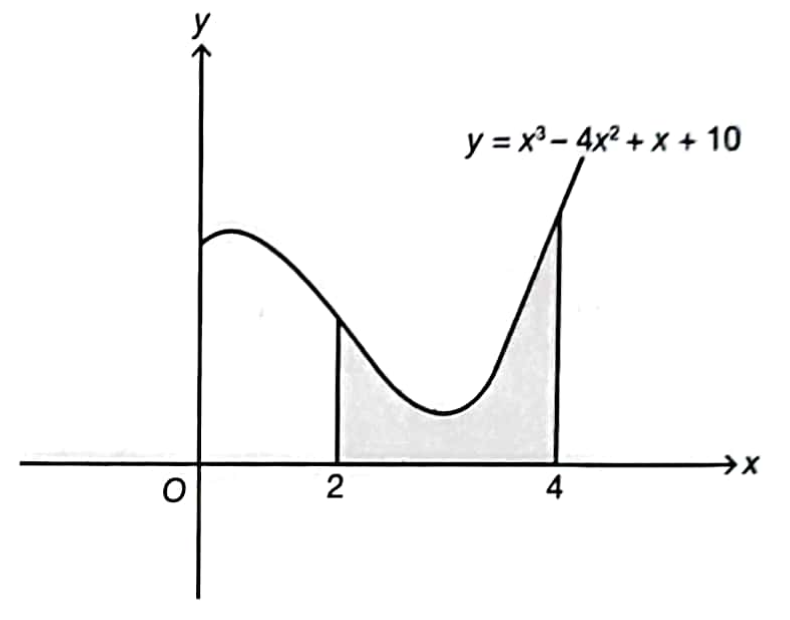
\includegraphics[width=0.3\textwidth,valign=t]{./images/1.png}
                              \sol{}
                              \begin{flalign*}
                                    A & = \int_2^4 (x^3 - 4x^2 + x + 10)\,dx                                                  \\
                                      & = \left[\frac{1}{4}x^4 - \frac{4}{3}x^3 + \frac{1}{2}x^2 + 10x\right]_2^4           & \\
                                      & = \left(64 - \frac{256}{3} + 8 + 40\right) - \left(4 - \frac{32}{3} + 2 + 20\right)   \\
                                      & = \frac{80}{3} - \frac{46}{3}                                                         \\
                                      & = 11\frac{1}{3}\text{ units}^2 \eos
                              \end{flalign*}

                        \item 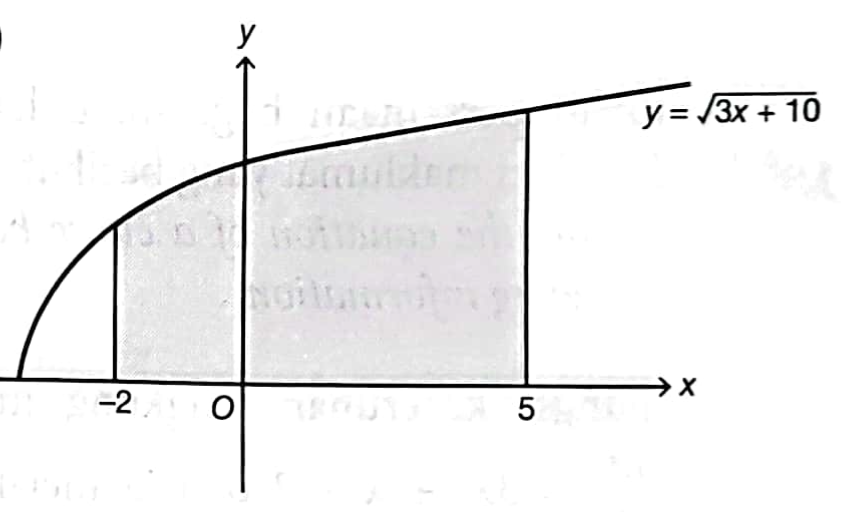
\includegraphics[width=0.3\textwidth,valign=t]{./images/2.png}
                              \sol{}
                              \begin{flalign*}
                                    A & = \int_{-2}^{5}\sqrt{3x+ 10}\,dx                                   \\
                                      & = \int_{-2}^{5}{(3x+10)}^{\frac{1}{2}}\,dx                         \\
                                      & = {\left[\frac{{2(3x + 10)}^{\frac{3}{2}}}{9}\right]}_{-2}^{5}     \\
                                      & = \frac{2{(25)}^{\frac{3}{2}}}{9} - \frac{2{(4)}^{\frac{3}{2}}}{9} \\
                                      & = \frac{250}{9} - \frac{16}{9}                                     \\
                                      & = \frac{234}{9}                                                    \\
                                      & = 26\text{ units}^2 \eos
                              \end{flalign*}

                        \item 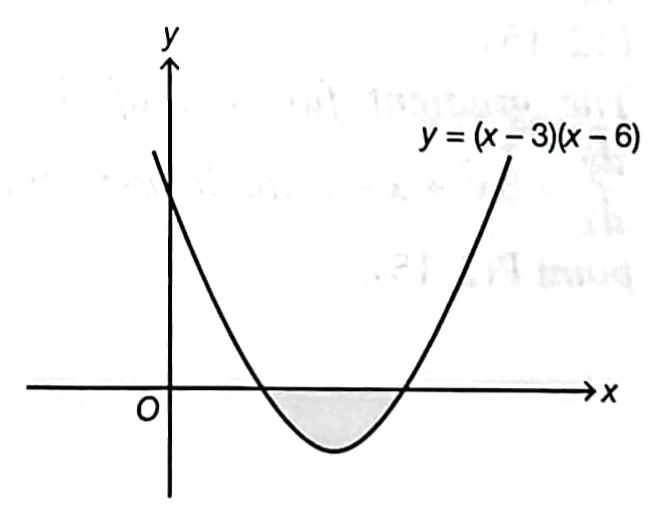
\includegraphics[width=0.3\textwidth,valign=t]{./images/3.png}
                              \sol{}
                              \begin{flalign*}
                                    A & = \left|\int_{3}^{6} (x-3)(x-6)\,dx                                        \right|   & \\
                                      & = \left|\int_{3}^{6} (x^2 - 9x + 18)\,dx                                     \right|   \\
                                      & = \left|{\left[\frac{1}{3}x^3 - \frac{9}{2}x^2 + 18x\right]}_3^6         \right|       \\
                                      & = \left|\left(72 - 162 + 108\right) - \left(9 - \frac{81}{2} + 54\right) \right|       \\
                                      & = \left|18 - \frac{45}{2}                                                \right|       \\
                                      & = 4.5\text{ units}^2 \eos
                              \end{flalign*}

                        \item 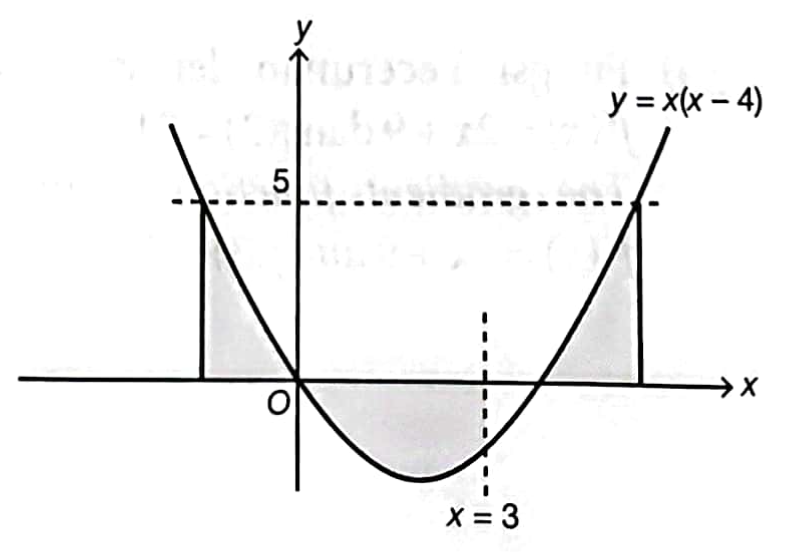
\includegraphics[width=0.3\textwidth,valign=t]{./images/4.png}
                              \sol{}

                              When $y = 5$,
                              \begin{flalign*}
                                    x(x-4)       & = 5               \\
                                    x^2 - 4x - 5 & = 0               \\
                                    (x-5)(x+1)   & = 0               \\
                                    x = -1       & \text{ or } x = 5
                              \end{flalign*}
                              When $y = 0$,
                              \begin{flalign*}
                                    x(x-4) & = 0               \\
                                    x = 0  & \text{ or } x = 4
                              \end{flalign*}
                              \begin{flalign*}
                                    A & = \int_{-1}^{0} x(x-4)\,dx + \left|\int_{0}^{3} x(x-4)\,dx\right|                                           \\
                                      & \ \ \ \ + \int_{4}^{5} x(x-4)\,dx                                                                         & \\
                                      & = \int_{-1}^{0} (x^2 - 4x)\,dx + \left|\int_{0}^{3} (x^2 - 4x)\,dx\right|                                   \\
                                      & \ \ \ \ + \int_{4}^{5} (x^2 - 4x)\,dx                                                                       \\
                                      & = {\left[\frac{1}{3}x^3 - 2x^2\right]}_{-1}^0 + \left|{\left[\frac{1}{3}x^3 - 2x^2\right]}_{0}^{3}\right|   \\
                                      & \ \ \ \ + {\left[\frac{1}{3}x^3 - 2x^2\right]}_{4}^5                                                        \\
                                      & = 0 - \left(-\frac{1}{3} - 2\right) + \left|\left(9 - 18\right) - 0\right|                                  \\
                                      & \ \ \ \ + \left(\frac{125}{3} - 50\right) - \left(\frac{64}{3} - 32\right)                                  \\
                                      & = 13\frac{2}{3}\text{ units}^2 \eos
                              \end{flalign*}
                  \end{enumerate}

            \item Determine the area bounded by the curve, the horizontal line(s) and the y-axis.
                  \begin{enumerate}
                        \item 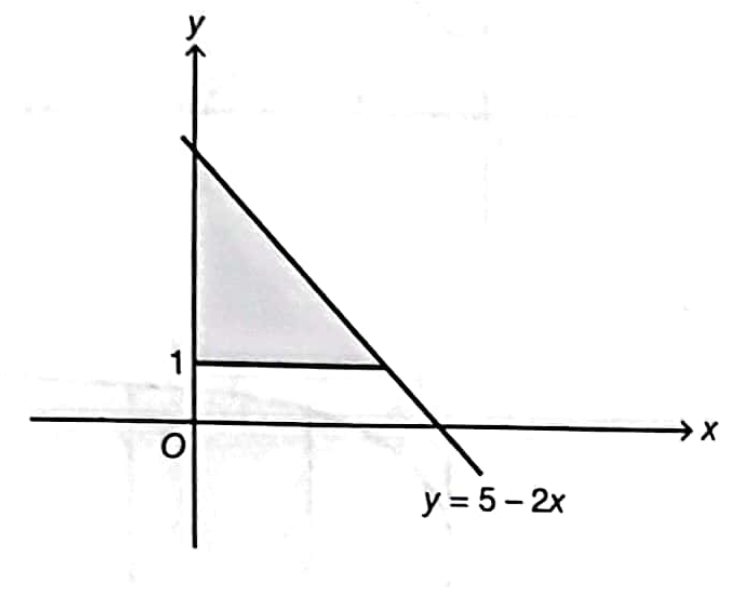
\includegraphics[width=0.3\textwidth,valign=t]{./images/5.png}
                              \sol{}
                              When $x = 0$,
                              \begin{flalign*}
                                    y  & = 5-2x          \\
                                    y  & = 5-2(0)        \\
                                       & = 5             \\
                                    \\
                                    y  & = 5-2x          \\
                                    2x & = 5 - y         \\
                                    x  & = \frac{5-y}{2}
                              \end{flalign*}
                              \begin{flalign*}
                                    A & = \int_1^5 \frac{5-y}{2}\,dy                                                        \\
                                      & =\int_1^5 \left(\frac{5}{2} - \frac{1}{2}y\right)\,dy                               \\
                                      & = {\left[\frac{5}{2}y - \frac{1}{4}y^2\right]}_1^5                                  \\
                                      & = \left(\frac{25}{2} - \frac{25}{4}\right) - \left(\frac{5}{2} - \frac{1}{4}\right) \\
                                      & = \frac{25}{4} - \frac{9}{4}                                                        \\
                                      & = 4\text{ units}^2 \eos
                              \end{flalign*}

                        \item 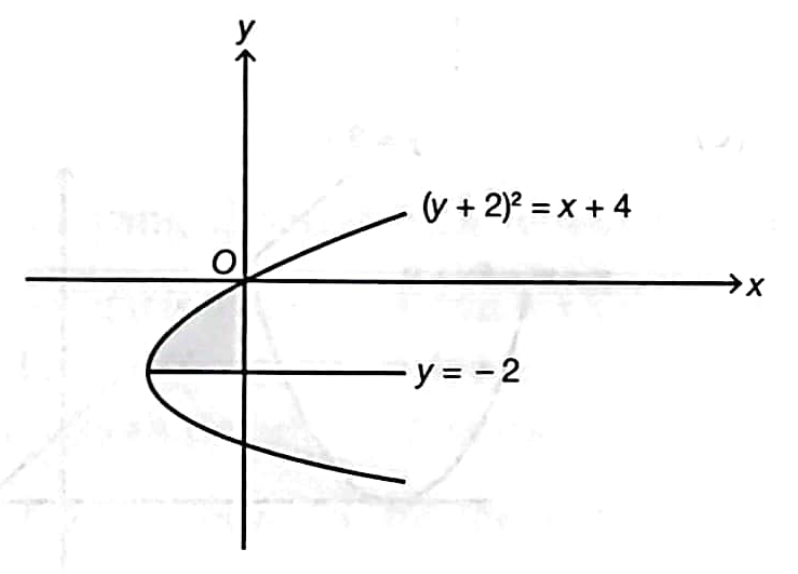
\includegraphics[width=0.3\textwidth,valign=t]{./images/6.png}
                              \sol{}
                              \begin{flalign*}
                                    {(y+2)}^2 & = x + 4            \\
                                    x         & = {(y+2)}^2 - 4    \\
                                              & = y^2 + 4y + 4 - 4 \\
                                              & = y^2 + 4y
                              \end{flalign*}
                              \begin{flalign*}
                                    A & = \int_{-2}^{0}(y^2 + 4y)\,dy                 \\
                                      & = {\left[\frac{1}{3}y^3 + 2y^2\right]}_{-2}^0 \\
                                      & = 0 - \left(-\frac{8}{3} + 8\right)           \\
                                      & = 5\frac{1}{3}\text{ units}^2 \eos
                              \end{flalign*}

                        \item 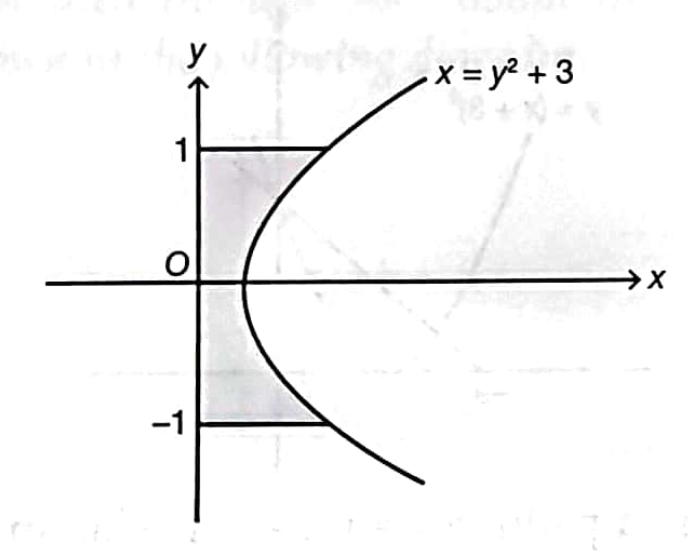
\includegraphics[width=0.3\textwidth,valign=t]{./images/7.png}
                              \sol{}
                              \begin{flalign*}
                                    A & = \int_{-1}^{1} (y^2 + 3)\,dy                                  \\
                                      & = {\left[\frac{1}{3}y^3 + 3y\right]}_{-1}^1                    \\
                                      & = \left(\frac{1}{3} + 3\right) - \left(-\frac{1}{3} - 3\right) \\
                                      & = 6\frac{2}{3}\text{ units}^2 \eos
                              \end{flalign*}

                        \item 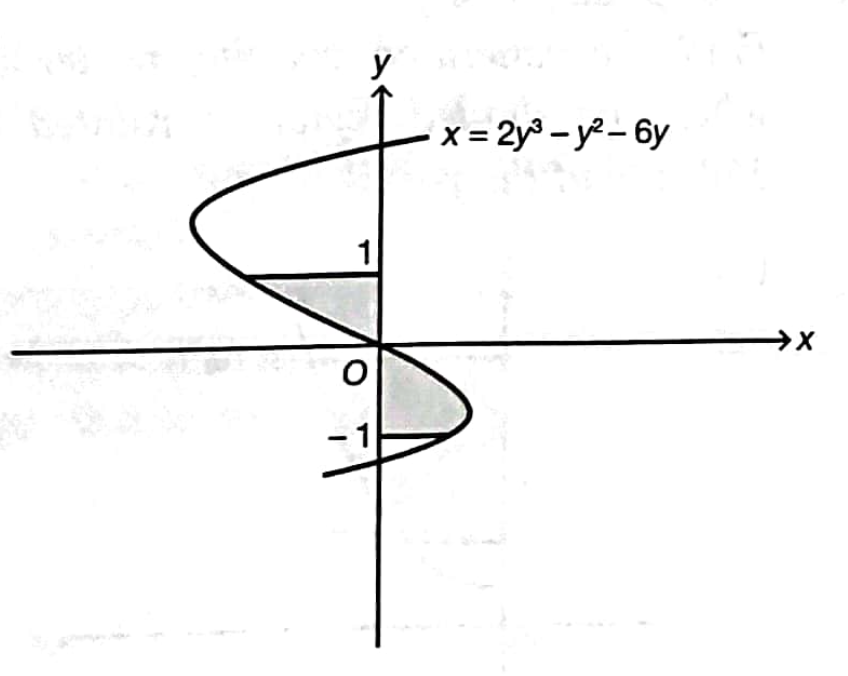
\includegraphics[width=0.3\textwidth,valign=t]{./images/8.png}
                              \sol{}
                              \begin{flalign*}
                                    A & = \int_{-1}^{0}(2y^3 - y^2 - 6y)\,dy + \left|\int_{0}^{1}(2y^3 - y^2 - 6y)\,dy\right|                                                     & \\
                                      & = {\left[\frac{1}{2}y^4 - \frac{1}{3}y^3 - 3y^2\right]}_{-1}^0 + \left|\left[\frac{1}{2}y^4 - \frac{1}{3}y^3 - 3y^2\right]_{0}^{1}\right|   \\
                                      & = 0 - \left(\frac{1}{2} + \frac{1}{3} - 3\right) + \left|\left(\frac{1}{2} - \frac{1}{3} - 3\right) - 0\right|                              \\
                                      & = \frac{13}{6} + \frac{17}{6}                                                                                                               \\
                                      & = 5\text{ units}^2 \eos
                              \end{flalign*}
                  \end{enumerate}

            \item Find the area of the shaded region for each of the following.
                  \begin{enumerate}
                        \item 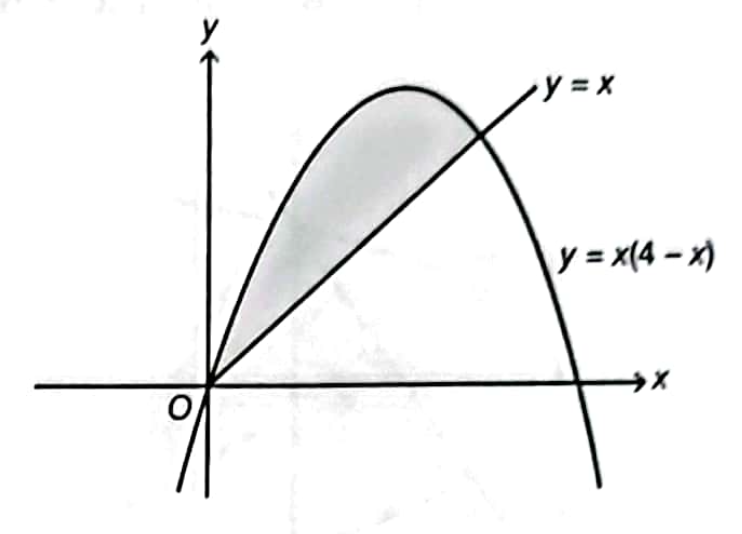
\includegraphics[width=0.3\textwidth,valign=t]{./images/9.png}
                              \sol{}
                              \begin{flalign*}
                                    x        & = x(4-x)          \\
                                    x        & = 4x - x^2        \\
                                    x^2 - 3x & = 0               \\
                                    x(x-3)   & = 0               \\
                                    x = 0    & \text{ or } x = 3
                              \end{flalign*}
                              \begin{flalign*}
                                    A & = \int_{0}^{3} \left[x(4-x) - x\right]\,dx           \\
                                      & = \int_{0}^{3} \left[4x - x^2 - x\right]\,dx         \\
                                      & = \int_{0}^{3} \left[3x - x^2\right]\,dx             \\
                                      & = {\left[\frac{3}{2}x^2 - \frac{1}{3}x^3\right]}_0^3 \\
                                      & = \left(\frac{27}{2} - 9\right) - 0                  \\
                                      & = 4.5\text{ units}^2 \eos
                              \end{flalign*}

                        \item 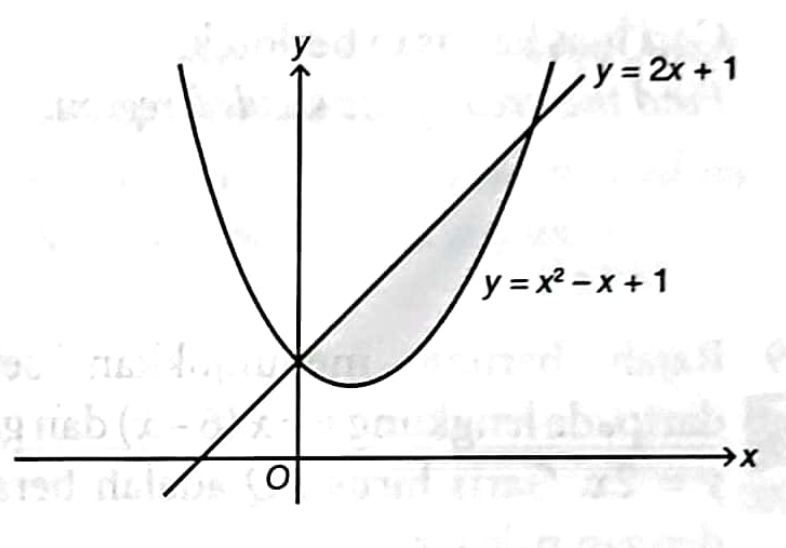
\includegraphics[width=0.3\textwidth,valign=t]{./images/10.png}
                              \sol{}
                              \begin{flalign*}
                                    2x + 1   & = x^2 - x + 1     \\
                                    x^2 - 3x & = 0               \\
                                    x(x-3)   & = 0               \\
                                    x = 0    & \text{ or } x = 3
                              \end{flalign*}
                              \begin{flalign*}
                                    A & = \int_0^3 \left[2x + 1 - x^2 + x - 1\right]\,dx      \\
                                      & = \int_0^3 \left[-x^2 + 3x\right]\,dx                 \\
                                      & = {\left[-\frac{1}{3}x^3 + \frac{3}{2}x^2\right]}_0^3 \\
                                      & = \left(-9 + \frac{27}{2}\right) - 0                  \\
                                      & = 4.5\text{ units}^2 \eos
                              \end{flalign*}

                        \item 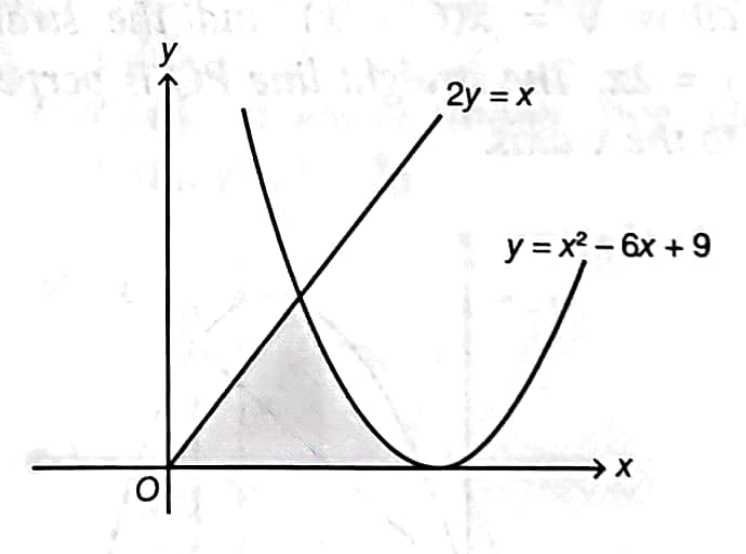
\includegraphics[width=0.3\textwidth,valign=t]{./images/11.png}
                              \sol{}
                              \begin{flalign*}
                                    2y              & = x                 \\
                                    y               & = \frac{1}{2}x      \\
                                    \frac{1}{2}x    & = x^2 - 6x + 9      \\
                                    x               & = 2x^2 - 12x + 18   \\
                                    2x^2 - 13x + 18 & = 0                 \\
                                    (2x - 9)(x - 2) & = 0                 \\
                                    x = 2           & \text{ or } x = 4.5 \\
                                    x^2 - 6x + 9    & = 0                 \\
                                    {(x-3)}^2       & = 0                 \\
                                    x               & = 3
                              \end{flalign*}
                              \begin{flalign*}
                                    A & = \int_{0}^{2} \frac{x}{2}\,dx + \int_{2}^{3} (x^2 - 6x + 9)\,dx                    \\
                                      & = {\left[\frac{1}{4}x^2\right]}_0^2 + {\left[\frac{1}{3}x^3 - 3x^2 + 9x\right]}_2^3 \\
                                      & = 1 - 0 + \left(9 - 27 + 27\right) - \left(\frac{8}{3} - 12 + 18\right)             \\
                                      & = 10 - \frac{26}{3}                                                                 \\
                                      & = 1\frac{1}{3}\text{ units}^2 \eos
                              \end{flalign*}

                        \item 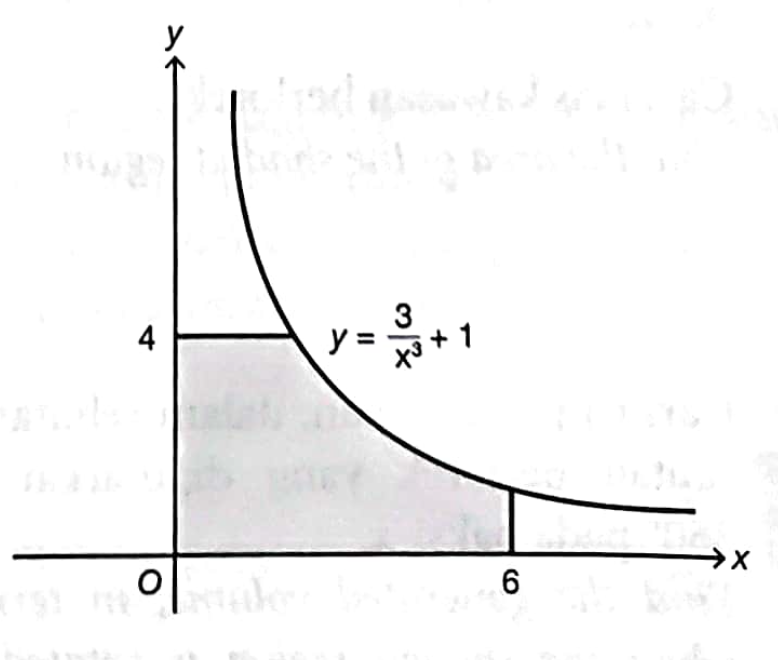
\includegraphics[width=0.3\textwidth,valign=t]{./images/12.png}
                              \sol{}
                              \begin{flalign*}
                                    \frac{3}{x^3} + 1 & =4  \\
                                    \frac{3}{x^3}     & = 3 \\
                                    x^3               & = 1 \\
                                    x                 & = 1
                              \end{flalign*}
                              \begin{flalign*}
                                    A & = 1 \cdot 4 + \int_1^6 \left(\frac{3}{x^3} + 1\right)\,dx            \\
                                      & = 4 + {\left[-\frac{3}{2x^2} + x\right]}_1^6                         \\
                                      & = 4 + \left(-\frac{1}{24} + 6\right) - \left(-\frac{3}{2} + 6\right) \\
                                      & = 4 + \frac{143}{24} + \frac{9}{2}                                   \\
                                      & = 14\frac{11}{24}\text{ units}^2 \eos
                              \end{flalign*}
                  \end{enumerate}

            \item The following diagram shows a part of the curve $x = y(y-6)$ and the straight
                  line $y = x+6$.
                  \begin{center}
                        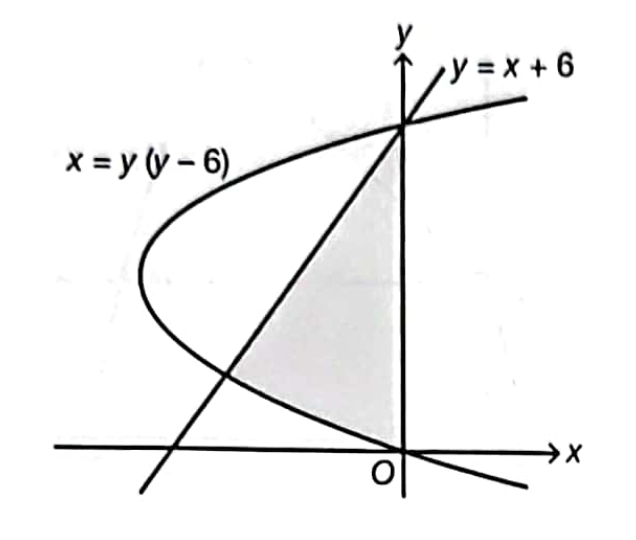
\includegraphics[width=0.3\textwidth,valign=t]{./images/13.png}
                  \end{center}
                  Find the area of the shaded region.
                  \sol{}
                  \begin{flalign*}
                        y                  & = x + 6           \\
                        x                  & = y - 6           \\
                        y - 6              & = y(y - 6)        \\
                                           & = y^2 - 6y        \\
                        y^2 - 7y + 6       & = 0               \\
                        (y - 6)(y - 1)     & = 0               \\
                        y              = 6 & \text{ or } y = 1 \\
                        1                  & = x + 6           \\
                        x                  & = -5
                  \end{flalign*}
                  \begin{flalign*}
                        A & = \left|\int_0^1 y(y-6)\,dy\right| + \frac{1}{2}(5)(5)                 \\
                          & = \left|\int_0^1 (y^2 - 6y)\,dy\right| + \frac{25}{2}                  \\
                          & = \left|{\left[\frac{1}{3}y^3 - 3y^2\right]}_0^1\right| + \frac{25}{2} \\
                          & = \left|\frac{1}{3} - 3 - 0\right| + \frac{25}{2}                      \\
                          & = \frac{8}{3} + \frac{25}{2}                                           \\
                          & = 15\frac{1}{6}\textit{ units}^2 \eos
                  \end{flalign*}

            \item The following diagram shows a part of the curve $y = x(6-x)$ and a straight
                  line $y = 2x$. The straight line $PQ$ is perpendicular to the x-axis.
                  \begin{center}
                        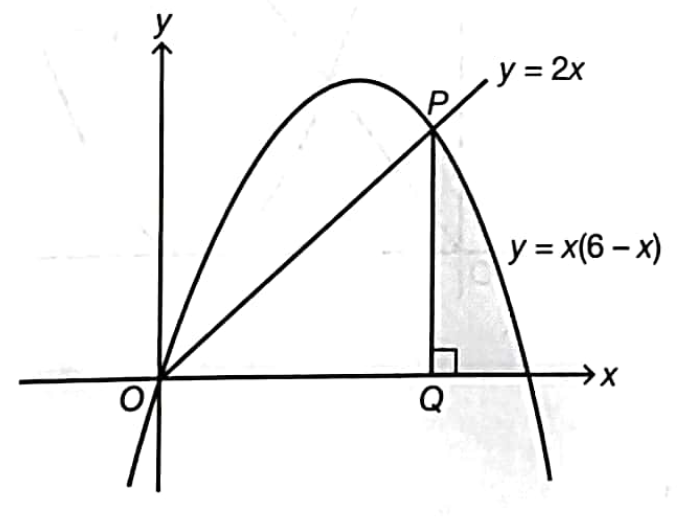
\includegraphics[width=0.3\textwidth,valign=t]{./images/14.png}
                  \end{center}
                  Find the area of the shaded region.
                  \sol{}
                  \begin{flalign*}
                        x(6 - x) & = 0               \\
                        x = 0    & \text{ or } x = 6 \\
                        2x       & = x(6-x)          \\
                        2x       & = 6x - x^2        \\
                        x^2 - 4x & = 0               \\
                        x(x - 4) & = 0               \\
                        x = 0    & \text{ or } x = 4 \\
                  \end{flalign*}
                  \begin{flalign*}
                        A & = \int_4^6 x(6-x)\,dx                                    \\
                          & = \int_4^6 (6x-x^2)\,dx                                  \\
                          & = {\left[3x^2 - \frac{1}{3}x^3\right]}_4^6               \\
                          & = \left(108 - 72\right) - \left(48 - \frac{64}{3}\right) \\
                          & = 36 - \frac{80}{3}                                      \\
                          & = 9\frac{1}{3}\textit{ units}^2 \eos
                  \end{flalign*}

            \item Find the generated volume, in terms of $\pi$, when the shaded region is rotated
                  through $360^{\circ}$ about the $x$-axis.
                  \begin{enumerate}
                        \item 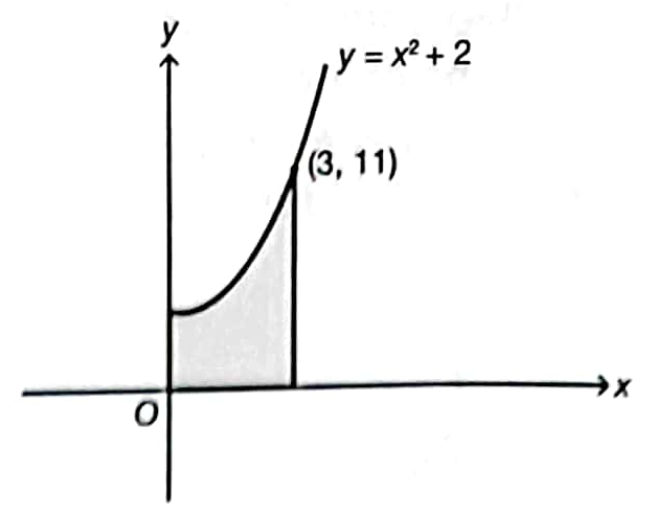
\includegraphics[width=0.3\textwidth,valign=t]{./images/15.png}
                              \sol{}
                              \begin{flalign*}
                                    V_x & = \int_0^3 \pi y^2\,dx                                       \\
                                        & = \pi\int_0^3 {(x^2 + 2)}^2\,dx                              \\
                                        & = \pi\int_0^3 (x^4 + 4x^2 + 4)\,dx                           \\
                                        & = \pi{\left[\frac{1}{5}x^5 + \frac{4}{3}x^3 + 4x\right]}_0^3 \\
                                        & = \left[\left(\frac{243}{5} + 36 + 12\right) - 0\right]\pi   \\
                                        & = 96.6\pi\textit{ units}^3 \eos
                              \end{flalign*}

                        \item 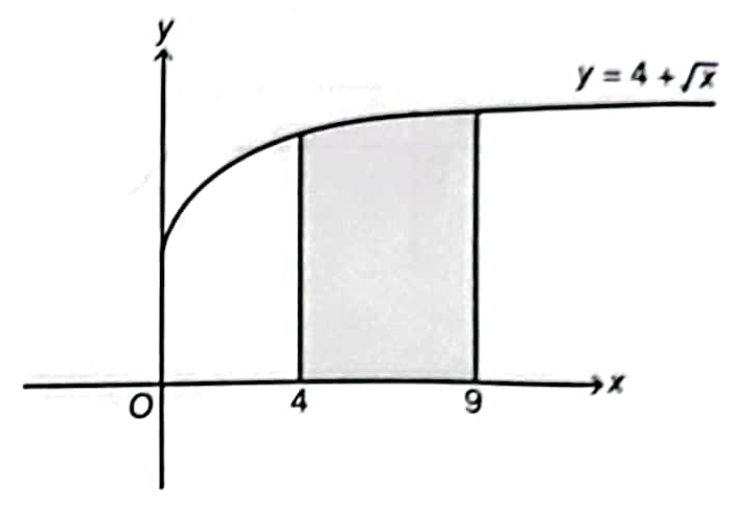
\includegraphics[width=0.3\textwidth,valign=t]{./images/16.png}
                              \sol{}
                              \begin{flalign*}
                                    V_x & = \int_4^9 \pi{(4+\sqrt{x})}^2\,dx                                                            & \\
                                        & = \pi\int_4^9 (16 + 8\sqrt{x} + x)\,dx                                                          \\
                                        & = \pi{\left[16x + \frac{16x^\frac{3}{2}}{3} + \frac{1}{2}x^2\right]}_4^9                        \\
                                        & = \pi\left[\left(144 + 144 + \frac{81}{2}\right) - \left(64 + \frac{128}{3} + 8\right)\right]   \\
                                        & = 213.83\pi\textit{ units}^3 \eos
                              \end{flalign*}

                        \item 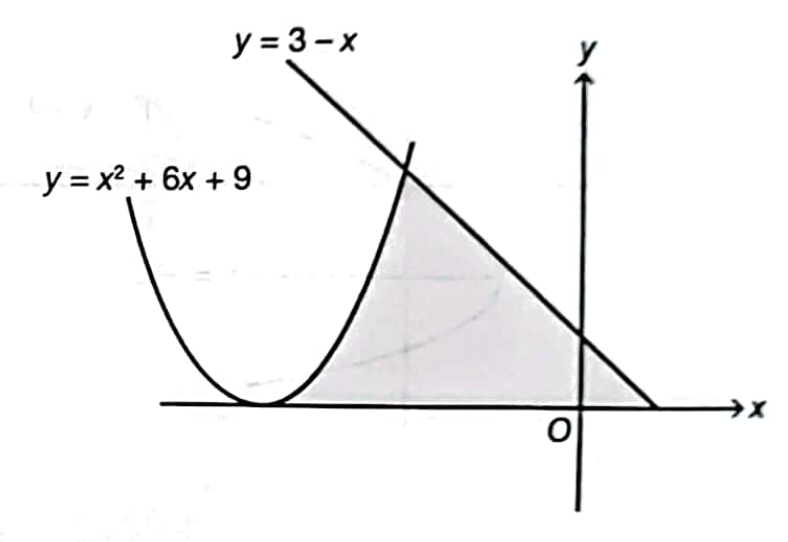
\includegraphics[width=0.3\textwidth,valign=t]{./images/17.png}
                              \sol{}
                              \begin{flalign*}
                                    x^2 + 6x + 9        & = 3-x              \\
                                    x^2 + 7x + 6        & = 0                \\
                                    (x + 6)(x + 1)      & = 0                \\
                                    x              = -6 & \text{ or } x = -1 \\
                                    x^2 + 6x + 9        & = 0                \\
                                    {(x + 3)}^2         & = 0                \\
                                    x                   & = -3               \\
                                    0                   & = 3-x              \\
                                    x                   & = 3
                              \end{flalign*}
                              \begin{flalign*}
                                    V_x & = \int_{-3}^{-1} \pi{(x+3)}^4\,dx + \int_{-1}^{3} \pi {(3-x)}^2\,dx                                             \\
                                        & =  \pi\int_{-3}^{-1} {(x+3)}^4\,dx + \pi\int_{-1}^{3} {(3-x)}^2\,dx                                             \\
                                        & = \pi\left\{{\left[\frac{{(x+3)}^5}{5}\right]}_{-3}^{-1} + {\left[-\frac{{(3-x)}^3}{3}\right]}_{-1}^{3}\right\} \\
                                        & = \pi\left[\left(\frac{32}{5} - 0\right) + \left(0 + \frac{64}{3}\right)\right]                                 \\
                                        & = 27\frac{11}{15}\pi \textit{ units}^3 \eos
                              \end{flalign*}

                        \item 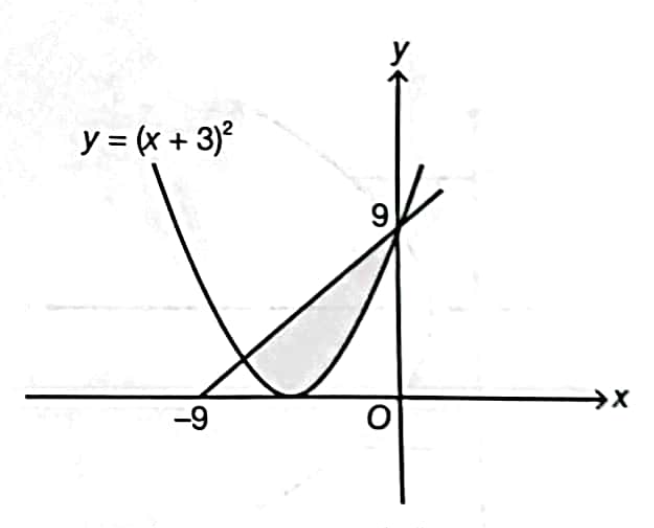
\includegraphics[width=0.3\textwidth,valign=t]{./images/18.png}
                              \sol{}

                              Let the line be $l$. Since $l$ passes through $(-9, 0)$ and $(0, 9)$,
                              \begin{flalign*}
                                    m_l          & = \dfrac{9}{9} = 1 \\
                                    y - 9        & = 1(x - 0)         \\
                                    y            & = x + 9            \\
                                    x + 9        & = {(x+3)}^2        \\
                                                 & = x^2 + 6x + 9     \\
                                    x^2 + 5x     & = 0                \\
                                    x(x+5)       & = 0                \\
                                    x        = 0 & \text{ or } x = -5
                              \end{flalign*}
                              \begin{flalign*}
                                    V_x & = \int_{-5}^{0} \pi{(x+9)}^2\,dx - \int_{-5}^{0} \pi{(x+3)}^4\,dx                                             \\
                                        & = \pi\int_{-5}^{0} {(x+9)}^2\,dx - \pi\int_{-5}^{0} {(x+3)}^4\,dx                                             \\
                                        & = \pi\left\{{\left[\frac{{(x+9)}^3}{3}\right]}_{-5}^{0} - {\left[\frac{{(x+3)}^5}{5}\right]}_{-5}^{0}\right\} \\
                                        & = \pi\left[\left(243 - \frac{64}{3}\right) - \left(\frac{243}{5} + \frac{32}{5}\right)\right]                 \\
                                        & = 116\frac{2}{3}\pi \textit{ units}^3 \eos
                              \end{flalign*}
                  \end{enumerate}

            \item Find the generated volume, in terms of $\pi$, when the shaded region is rotated
                  through $360^\circ$ about the y-axis.
                  \begin{enumerate}
                        \item 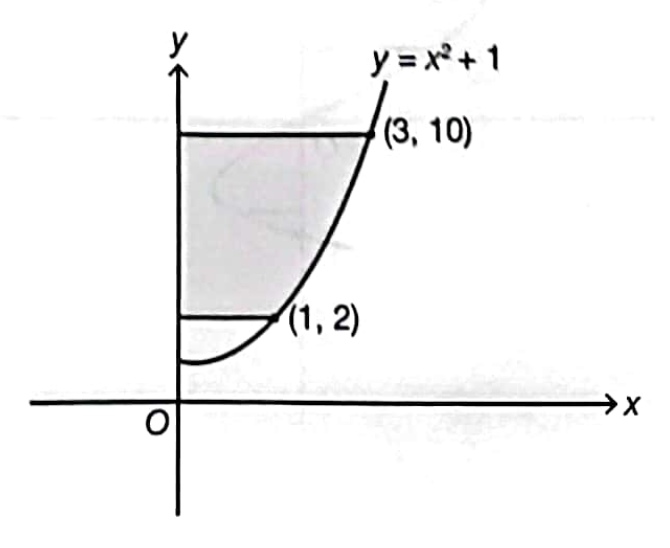
\includegraphics[width=0.3\textwidth,valign=t]{./images/19.png}
                              \sol{}
                              \begin{flalign*}
                                    y   & = x^2 + 1        \\
                                    x^2 & = y - 1          \\
                                    x   & - \sqrt{y-1} = 0
                              \end{flalign*}
                              \begin{flalign*}
                                    V_y & = \int_{2}^{10} \pi{(\sqrt{y-1})}^2\,dy                     \\
                                        & = \pi\int_{2}^{10} y-1\,dy                                  \\
                                        & = \pi{\left[\frac{y^2}{2} - y\right]}_2^{10}                \\
                                        & = \pi\left[\left(50 - 10\right) - \left(2 - 2\right)\right] \\
                                        & = 40\pi \textit{ units}^3 \eos
                              \end{flalign*}

                        \item 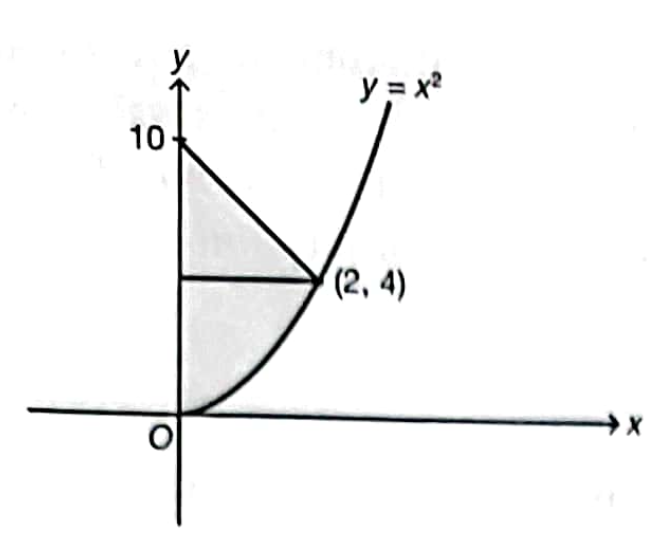
\includegraphics[width=0.3\textwidth,valign=t]{./images/20.png}
                              \sol{}
                              \begin{flalign*}
                                    y & = x^2      \\
                                    x & = \sqrt{y}
                              \end{flalign*}
                              \begin{flalign*}
                                    V_y & = \int_{0}^{4} \pi {\left(\sqrt{y}\right)}^2\,dy + \frac{1}{3} \pi \cdot 4 \cdot 6 \\
                                        & = \pi\int_{0}^{4} y\,dy + 8\pi                                                     \\
                                        & = \pi{\left[\frac{y^2}{2}\right]}_0^4 + 8\pi                                       \\
                                        & = 8\pi + 8\pi                                                                      \\
                                        & = 16\pi \textit{ units}^3 \eos
                              \end{flalign*}

                        \item 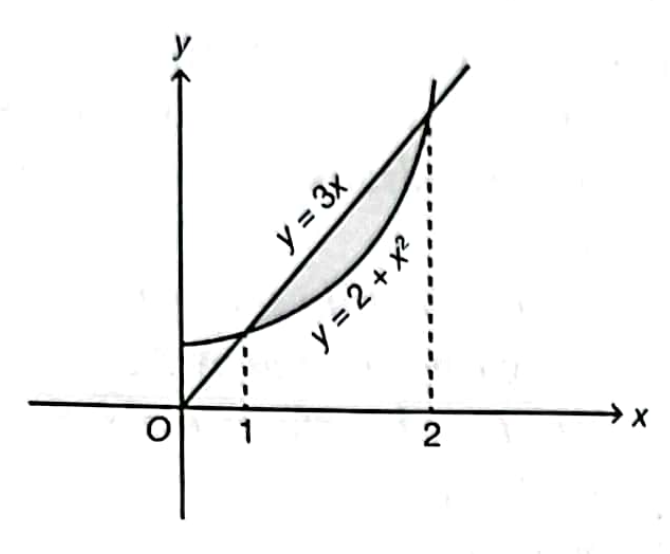
\includegraphics[width=0.3\textwidth,valign=t]{./images/21.png}
                              \sol{}
                              \begin{flalign*}
                                    y         & = 3x           \\
                                    x         & = \dfrac{y}{3} \\
                                    y         & = 2 + x^2      \\
                                    x^2       & = y - 2        \\
                                    x         & = \sqrt{y - 2} \\
                                    x = 1,\ y & = 3(1) = 3     \\
                                    x = 2,\ y & = 3(2) = 6
                              \end{flalign*}
                              \begin{flalign*}
                                    V_y & = \int_3^6 \pi {\left(\sqrt{y - 2}\right)}^2\,dy - \int_3^6 \pi {\left(\frac{y}{3}\right)}^2\,dy & \\
                                        & = \pi\int_3^6  {(y - 2)}\,dy - \pi\int_3^6 {\frac{y^2}{9}}\,dy                                     \\
                                        & = \pi{\left[\frac{y^2}{2} - 2y\right]}_3^6 - \pi{\left[\frac{y^3}{27}\right]}_3^6                  \\
                                        & = \pi{\left\{\left[(18 - 12) - \left(\frac{9}{2} - 6\right)\right] - \left(8 - 1\right)\right\}}   \\
                                        & = \pi\left(\frac{15}{2} - 7\right)                                                                 \\
                                        & = \frac{1}{2} \pi\textit{ units}^3 \eos
                              \end{flalign*}
                  \end{enumerate}

            \item The region bounded by the curve $y = \dfrac{8}{x}$, the x-axis, and the
                  straight line $x = 2$ and $x = k$ is rotated through $360^\circ$ about the
                  x-axis as shown in the following diagram.
                  \begin{center}
                        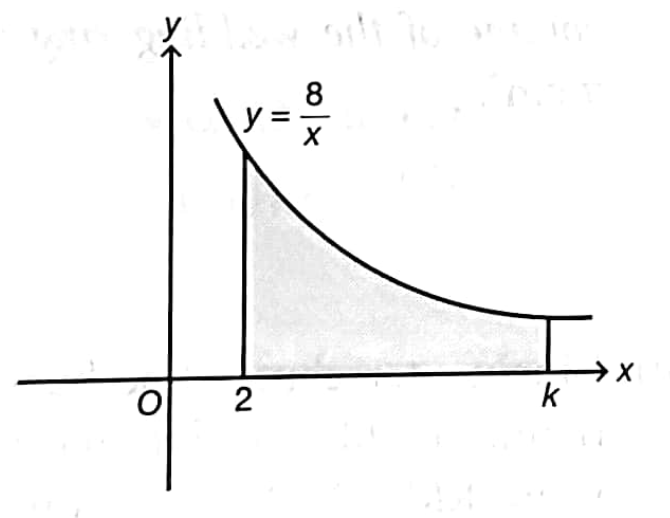
\includegraphics[width=0.3\textwidth,valign=t]{./images/22.png}
                  \end{center}
                  Express the volume generated by the region in terms of $k$. If the value of $k$ becomes extremely large, deduce the nearest value of volume.
                  \begin{flalign*}
                        V_x & = \int_2^k \pi{\left(\frac{8}{x}\right)}^2\,dx \\
                            & = \pi\int_2^k \frac{64}{x^2}\,dx               \\
                            & = \pi{\left[-\frac{64}{x}\right]}_2^k          \\
                            & = -\frac{64\pi}{k} + 32\pi \eos
                  \end{flalign*}
                  \begin{flalign*}
                        k            & \to \infty \Rightarrow \frac{1}{k} \approx 0 \\
                        \therefore\  & V_x \approx 32 \textit{ units}^3 \eos
                  \end{flalign*}

            \item The following diagram shows a part of the curve $y =4 +3x - x^2$ and the
                  straight line $y = x+1$.
                  \begin{center}
                        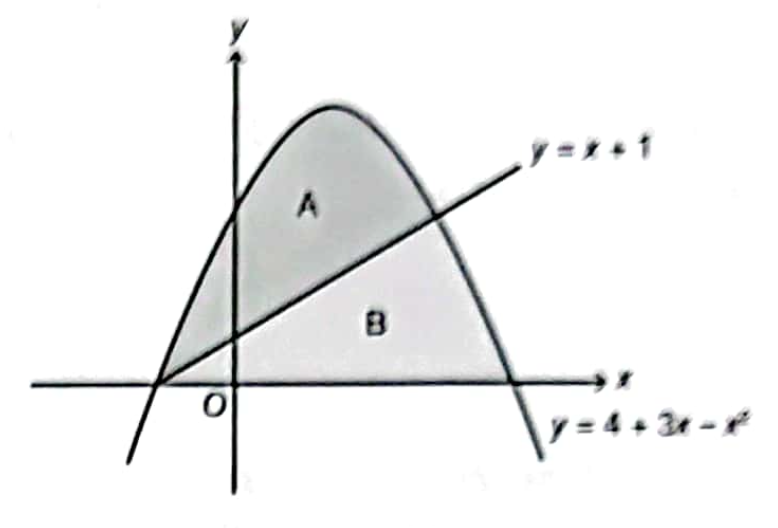
\includegraphics[width=0.33 \textwidth,valign=t]{./images/23.png}
                  \end{center}
                  Find the ratio of the area of the shaded region $A$ to the area of the shaded region $B$.
                  \sol{}
                  \begin{flalign*}
                        x + 1         & = 4 + 3x - x^2    \\
                        -x^2 + 2x + 3 & = 0               \\
                        x^2 - 2x - 3  & = 0               \\
                        (x-3)(x+1)    & = 0               \\
                        x = 3         & \text{ or }x = -1 \\
                        x = 3,\ y     & = 3 + 1 = 4
                  \end{flalign*}
                  \begin{flalign*}
                        A_A & = \int_{-1}^3 (4+3x-x^2)\,dx - \frac{1}{2} \cdot 4 \cdot 4                             \\
                            & = {\left[4x + \frac{3}{2}x^2 - \frac{1}{3}x^3\right]}_{-1}^3 - 8                       \\
                            & = \left(12 + \frac{27}{2} - 9\right) - \left(-4 + \frac{3}{2} + \frac{1}{3}\right) - 8 \\
                            & = \frac{33}{2} + \frac{13}{6} - 8                                                      \\
                            & = \frac{32}{3} \textit{ units}^2
                  \end{flalign*}
                  \begin{flalign*}
                        4 + 3x - x^2 & = 0               \\
                        x^2 - 3x - 4 & = 0               \\
                        (x-4)(x+1)   & = 0               \\
                        x = 4        & \text{ or }x = -1 \\
                  \end{flalign*}
                  \begin{flalign*}
                        A_B & = \int_{3}^4 (4+3x-x^2)\,dx + \frac{1}{2} \cdot 4 \cdot 4                      \\
                            & = {\left[4x + \frac{3}{2}x^2 - \frac{1}{3}x^3\right]}_{3}^4 + 8                \\
                            & = \left(16 + 24 - \frac{64}{3}\right) - \left(12 + \frac{27}{2} - 9\right) + 8 \\
                            & = \frac{56}{3} - \frac{33}{2} + 8                                              \\
                            & = \frac{61}{6} \textit{ units}^2
                  \end{flalign*}
                  \begin{flalign*}
                        \therefore\ A_A : A_B & = \frac{32}{3} : \frac{61}{6} \\
                                              & = \frac{64}{61}               \\
                                              & = 64 : 61 \eos
                  \end{flalign*}

            \item The following diagram shows two curves $y = x^2 - 1$ and $y = 3+2x-x^2$.
                  \begin{center}
                        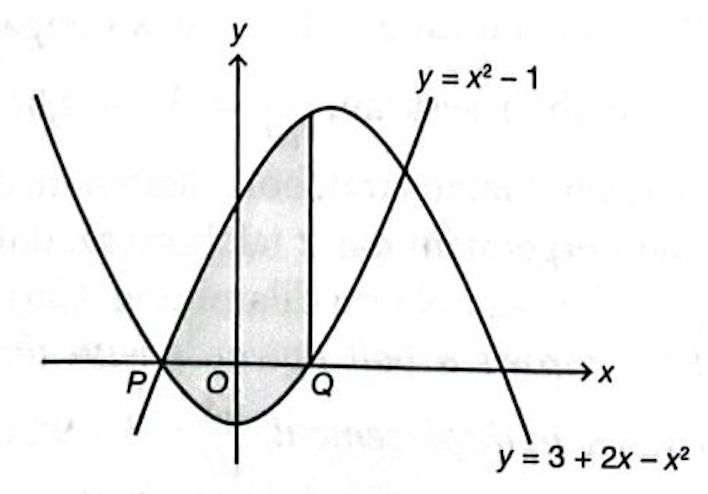
\includegraphics[width=0.3\textwidth,valign=t]{./images/24.png}
                  \end{center}
                  Find the coordinate of the points $P$ and $Q$. Hence, calculate the area of the shaded region.
                  \sol{}
                  \begin{flalign*}
                        x^2 - 1    & = 0               \\
                        (x+1)(x-1) & = 0               \\
                        x = -1     & \text{ or }x = 1  \\
                        \\
                        3+2x-x^2   & = 0               \\
                        (x-3)(x+1) & = 0               \\
                        x = 3      & \text{ or }x = -1
                  \end{flalign*}
                  Since $y = x^2 - 1$ and $y = 3+2x-x^2$ intersect at $x = -1$, $P(-1,0)$. $\eos$

                  Since another root of $y = x^2 - 1$ is $1$, $Q(1,0)$. $\eos$
                  \begin{flalign*}
                        A & = \left|\int_{-1}^1 (x^2 - 1)\,dx\right| + \int_{-1}^1 (3+2x-x^2)\,dx                                          \\
                          & = \left|{\left[\frac{1}{3}x^3 - x\right]}_{-1}^1\right| + {\left[3x + x^2 - \frac{1}{3}x^3\right]}_{-1}^1      \\
                          & = \left|\left(\frac{1}{3} - 1\right) - \left(-\frac{1}{3} + 1\right)\right| + \left(3 + 1 - \frac{1}{3}\right) \\
                          & \ \ \ \ - \left(-3 + 1 + \frac{1}{3}\right)                                                                    \\
                          & = \frac{4}{3} + \frac{11}{3} + \frac{5}{3}                                                                     \\
                          & = 6\frac{2}{3} \textit{ units}^2 \eos
                  \end{flalign*}

            \item Calculate the volume generated, in terms of $\pi$, when the region bound by the
                  curve $y = 3x^2$, the straight line $x = 1$ and $x = 4$ and the x-axis is
                  rotated through two right angles about the x-axis. \sol{}
                  \begin{flalign*}
                        V_x & = \frac{1}{2}\int_1^4 \pi{(3x^2)}^2\,dx                   \\
                            & = \frac{1}{2}\pi\int_1^4 (9x^4)\,dx                       \\
                            & = \frac{1}{2}\pi{\left[\frac{9}{5}x^5\right]}_1^4         \\
                            & = \frac{1}{2}\pi\left(\frac{9216}{5} - \frac{9}{5}\right) \\
                            & = 920\frac{7}{10}\pi \textit{ units}^3 \eos
                  \end{flalign*}
      \end{enumerate}

      \section{Application of Integration}

      \begin{enumerate}
            \setcounter{enumi}{26}

            \item A container is filled with water. After $t$ seconds, the height of the water,
                  $h$\textit{cm}, in the containers increases at the rate of
                  $0.56t\textit{cm}\textit{s}^{-1}$. Given that the container is empty when $t =
                        0$, find the value of $t$ when $h = 28$. \sol{}
                  \begin{flalign*}
                        \frac{dh}{dt}          & = 0.56t                           \\
                        \int \frac{dh}{dt}\,dt & = \int 0.56t\,dt                  \\
                        h                      & = 0.28t^2 + C                     \\
                        \because\ t            & = 0 \text{ when } h = 0           \\
                        \therefore\ C          & = 0                               \\
                        h                      & = 0.28t^2                         \\
                        0.28t^2                & = 28                              \\
                        0.01t^2                & = 1                               \\
                        t^2                    & = 100                             \\
                        t                      & = 10\textit{s} \quad (t > 0) \eos
                  \end{flalign*}

            \item Raja throws a ball upwards with the rate of change in displacement,
                  $\dfrac{ds}{dt} = 3 - 9.8t$, where $s$ is the displacement, in \textit{m}, of
                  the ball from the initial point and $t$ is the time, in seconds, the moment the
                  ball is thrown upwards. Find \sol{}
                  \begin{flalign*}
                        \frac{ds}{dt}          & = 3 - 9.8t            \\
                        \int \frac{ds}{dt}\,dt & = \int (3 - 9.8t)\,dt \\
                        s                      & = 3t - 4.9t^2 + C     \\
                        \because\ t            & = 0,\ s = 0           \\
                        \therefore\ C          & = 0                   \\
                        s                      & = 3t - 4.9t^2
                  \end{flalign*}
                  \begin{enumerate}
                        \item the maximum height, in $m$, achieved by the ball. \sol{} $\dfrac{ds}{dt} = 0$
                              when the ball is at its maximum height.
                              \begin{flalign*}
                                    3 - 9.8t & = 0                                                               \\
                                    9.8t     & = 3                                                               \\
                                    t        & = \frac{15}{49}\textit{s}                                         \\
                                    s        & = 3\left(\frac{15}{49}\right) - 4.9{\left(\frac{15}{49}\right)}^2 \\
                                             & = \frac{45}{98} \eos
                              \end{flalign*}

                        \item the time taken, in seconds, for the ball to return to its initial point. \sol{}
                              \begin{flalign*}
                                    s           & = 0                                     \\
                                    3t - 4.9t^2 & = 0                                     \\
                                    t(3-4.9t)   & = 0                                     \\
                                    t = 0       & \text{ or } t = \frac{30}{49}\textit{s}
                              \end{flalign*}
                              Therefore, the time taken for the ball to return to its initial point is $\dfrac{30}{49}$ seconds.
                  \end{enumerate}

            \item The following diagram shows the cross section of a wedding ring ordered by
                  Azmin. The inner and outer curved surfaces are represented by the quadratic
                  equations of $x = 0.8 - 0.5y^2$ and $x = 1 - y^2$ respectively.
                  \begin{center}
                        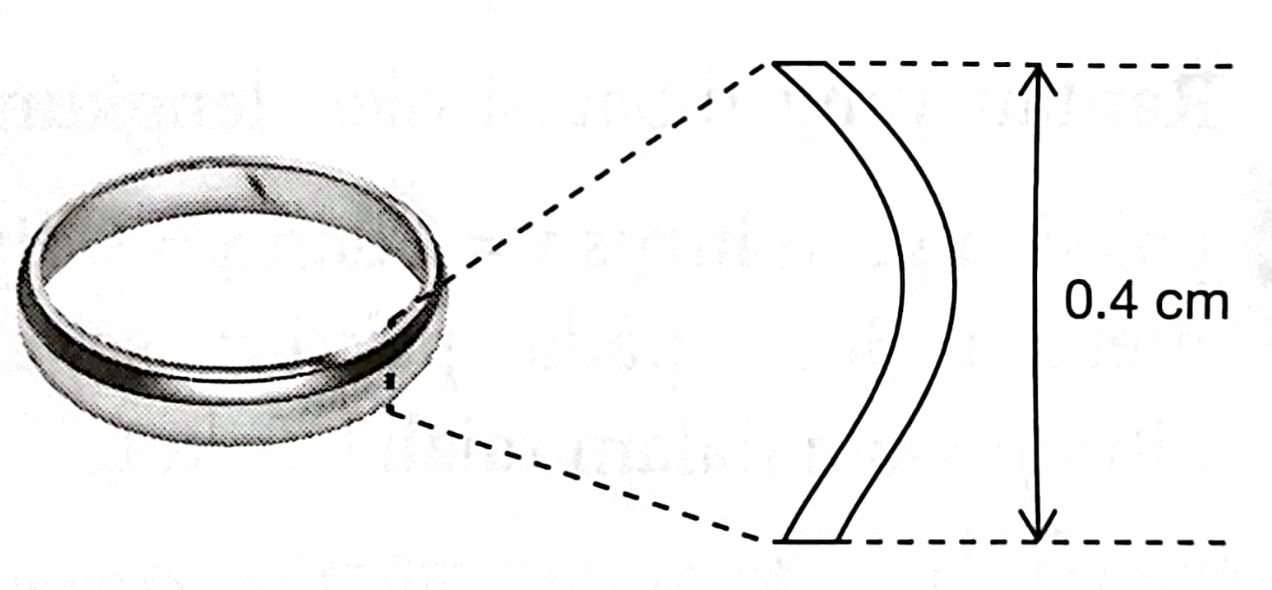
\includegraphics[width=0.35\textwidth]{./images/25.png}
                  \end{center}
                  \begin{enumerate}
                        \item By using the calculus method, find the volume of the wedding ring in terms of
                              $\pi \textit{cm}^3$. \sol{}
                              \begin{flalign*}
                                    V_x & = \int_{-0.2}^{0.2} \pi\left[{(1-y^2)}^2 - {(0.8-0.5y^2)}^2\right]\,dy                                                        & \\
                                        & = \pi\int_{-0.2}^{0.2} \left[(1 - 2y^2 + y^4) - (0.64 - 0.8y^2 \right.                                                          \\
                                        & \ \ \ \ \left.+ 0.25y^4)\right]\,dy                                                                                             \\
                                        & = \pi\int_{-0.2}^{0.2} \left[0.36 -1.2y^2 + 0.75y^4\right]\,dy                                                                  \\
                                        & = \pi\int_{-\frac{1}{5}}^{\frac{1}{5}} \left[\frac{9}{25} -\frac{6}{5}y^2 + \frac{3}{4}y^4\right]\,dy                           \\
                                        & = \pi{\left[\frac{9}{25}y - \frac{2}{5}y^3 + \frac{3}{20}y^5\right]}_{-\frac{1}{5}}^{\frac{1}{5}}                               \\
                                        & = \pi\left[\left(\frac{9}{125} - \frac{2}{625} + \frac{3}{62500}\right) - \left(-\frac{9}{125} + \frac{2}{625} \right.\right.   \\
                                        & \ \ \ \ \left.\left.- \frac{3}{62500}\right)\right]                                                                             \\
                                        & = \pi\left(\frac{4303}{62500} + \frac{4303}{62500}\right)                                                                       \\
                                        & = 0.1377\pi \textit{cm}^3 \eos
                              \end{flalign*}

                        \item The ring is made of titanium. If the rate of price of titanium is RM$153.49$
                              per gram and the rate of titanium mass per unit volume is
                              $4.51\textit{g}\textit{cm}^{-3}$, calculate the price needed to be paid by
                              Azmin. (Use $\pi = 3.142$). \sol{}
                              \begin{flalign*}
                                    \text{Mass}  & = 4.51\textit{g}\textit{cm}^{-3} \times 0.1377\pi \textit{cm}^3 \\
                                                 & = 1.9513\textit{g}                                              \\
                                    \text{Price} & = \text{RM}153.49\textit{g}^{-1} \times 1.9513\textit{g}        \\
                                                 & = \text{RM}299.51 \eos
                              \end{flalign*}
                  \end{enumerate}
      \end{enumerate}
\end{multicols*}
\begin{multicols*}{2}
      \noindent\Large{\underline{\textbf{Praktis Summatif}}}
      \normalsize
      \setcounter{section}{0}
      \section{Kertas 1}

      \begin{enumerate}
            \item Given that $\displaystyle \int_m^2(2x+3)\,dx = -8$ where $m > 0$, find the
                  value of $m$. \sol{}
                  \begin{flalign*}
                        \int_m^2(2x+3)\,dx & = \left[x^2 + 3x\right]_m^2 \\
                                           & = 4 + 6 - m^2 - 3m          \\
                                           & = 10 - 3m - m^2             \\
                        10 - 3m - m^2      & = -8                        \\
                        m^2 + 3m - 10      & = 8                         \\
                        m^2 + 3m - 18      & = 0                         \\
                        (m+6)(m-3)         & = 0                         \\
                        m                  & = 3 \quad (m > 0) \eos
                  \end{flalign*}

            \item Given that $\dfrac{dy}{dx} = 10{(5x + 3)}^2$ and $y = 4$ when $x = 0$. Express
                  $y$ in terms of $x$.

            \item Given $\displaystyle \int_5^m f(t)\,dx = \dfrac{7}{3}$, find
                  \begin{enumerate}
                        \item $\displaystyle \int_m^5 3f(t)\,dx  = \dfrac{7}{3}$.
                              \sol{}
                              \begin{flalign*}
                                    \int_m^5 3f(t)\,dx & = -\int_5^m 3f(t)\,dx \\
                                                       & = -3\int_5^m f(t)\,dx \\
                                                       & = -3\dfrac{7}{3}      \\
                                                       & = -7 \eos
                              \end{flalign*}

                        \item the value of $m$, where $\displaystyle \int_5^m [4-f(t)]\,dx = 7$. \sol{}
                              \begin{flalign*}
                                    \int_5^m [4-f(t)]\,dx               & = 7            \\
                                    \int_5^m 4\,dx - \int_5^m f(t)\,dx  & = 7            \\
                                    {\left[4x\right]}_5^m - \frac{7}{3} & = 7            \\
                                    4m - 20                             & = \frac{28}{3} \\
                                    12m - 60                            & = 28           \\
                                    12m                                 & = 88           \\
                                    m                                   & = 7\frac{1}{3}
                              \end{flalign*}
                  \end{enumerate}

            \item Given that $\displaystyle \int \dfrac{3}{{(3x-2)}^n}\,dx = a{(3x-2)}^{1-n} +
                        C$,
                  \begin{enumerate}
                        \item State the impossible value of $n$. \sol{}
                              \begin{flalign*}
                                    \int \dfrac{3}{{(3x-2)}^n}\,dx & = 3\int {(3x-2)}^{-n}\,dx                          & \\
                                                                   & = 3\left[\dfrac{{(3x-2)}^{1-n}}{3(1-n)}\right] + C   \\
                                                                   & = \dfrac{{(3x-2)}^{1-n}}{1-n} + C                    \\
                                    a{(3x-2)}^{1-n} + C            & = \dfrac{1}{1-n}{(3x-2)}^{1-n} + C
                              \end{flalign*}
                              Comparing both sides,
                              \begin{flalign*}
                                    a & = \frac{1}{1-n}
                              \end{flalign*}
                              $a$ is undefined when $1-n = 0$.
                              \begin{flalign*}
                                    1 - n & = 0 \\
                                    n     & = 1
                              \end{flalign*}
                              Therefore, $n = 1$ is impossible. $\eos$

                        \item Hence, express $n$ in terms of $a$. \sol{}
                              \begin{flalign*}
                                    a      & = \frac{1}{1-n}      \\
                                    a(1-n) & = 1                  \\
                                    a - an & = 1                  \\
                                    an     & = a - 1              \\
                                    n      & = \frac{a-1}{a} \eos
                              \end{flalign*}
                  \end{enumerate}

            \item Diagram below shows a curve $y = f(x)$.
                  \begin{center}
                        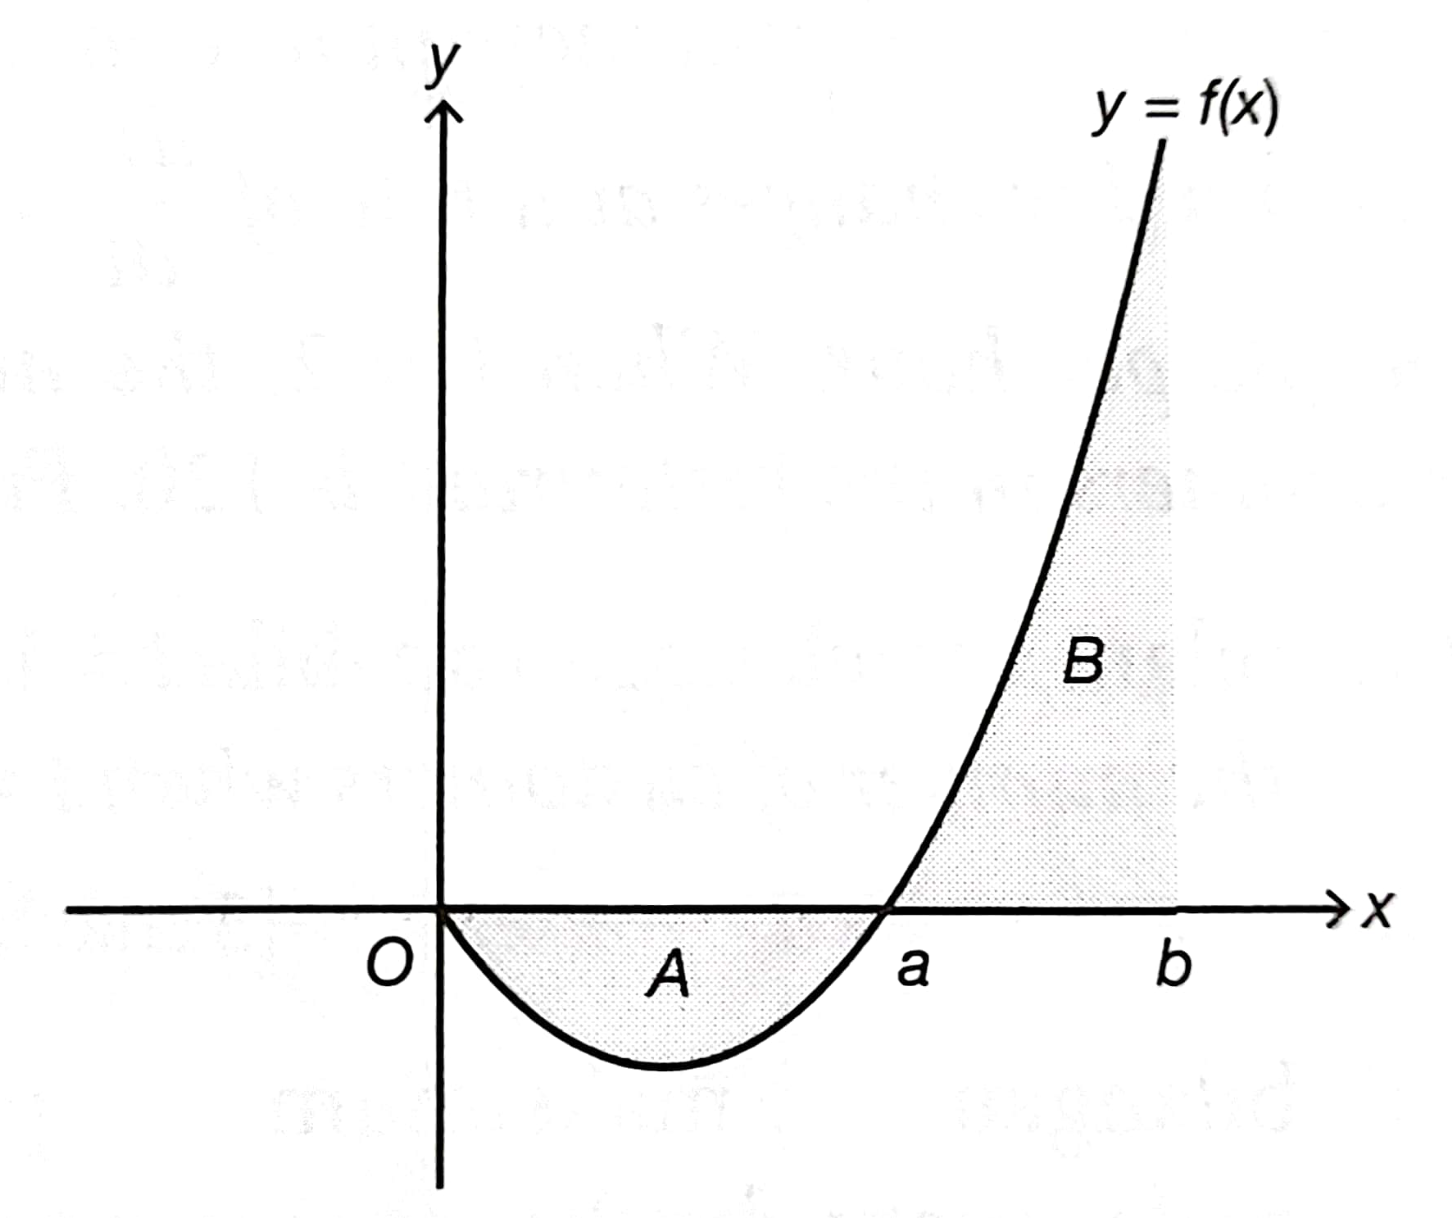
\includegraphics[width=0.35\textwidth]{images/26.png}
                  \end{center}
                  Given area of region $B$ is three times the area of region $A$ and
                  $\displaystyle \int_0^b f(x)\,dx = 20$, find the area of region $B$.
                  \sol{}
                  \begin{flalign*}
                        \int_0^b f(x)\,dx & = \int_0^a f(x)\,dx + \int_a^b f(x)\,dx             \\
                        20                & = -\int_0^a f(x)\,dx + \int_a^b f(x)\,dx            \\
                        20                & = -\frac{1}{3}\int_a^b f(x)\,dx + \int_a^b f(x)\,dx \\
                        20                & = -\frac{1}{3}A_B + A_B                             \\
                        20                & = \frac{2}{3}A_B                                    \\
                        2A_B              & = 60                                                \\
                        A_B               & = 30 \eos
                  \end{flalign*}
      \end{enumerate}

      \section{Kertas 2}
      \begin{enumerate}
            \item Differentiate $2x^4\sqrt{4x-3}$ with respect to $x$. Hence, find $\displaystyle
                        \int \dfrac{3x^4 - 2x^3}{\sqrt{4x-3}}\,dx$. \sol{}
                  \begin{flalign*}
                        \frac{dy}{dx}(2x^4\sqrt{4x-3})            & = 8x^3\sqrt{4x-3} + 2x^4\left(\frac{4}{2\sqrt{4x-3}}\right) & \\
                                                                  & = 8x^3\sqrt{4x-3} + \frac{4x^4}{\sqrt{4x-3}}                  \\
                                                                  & = \frac{8x^3(4x-3) + 4x^4}{\sqrt{4x-3}}                       \\
                                                                  & = \frac{4x^3(8x -6 +x)}{\sqrt{4x-3}}                          \\
                                                                  & = \frac{12(3x^4 - 2x^3)}{\sqrt{4x-3}} \eos                    \\
                        \\
                        \int \dfrac{3x^4 - 2x^3}{\sqrt{4x-3}}\,dx & = \frac{1}{12}\int \frac{12(3x^4 - 2x^3)}{\sqrt{4x-3}}\,dx    \\
                                                                  & = \frac{1}{12}\cdot 2x^4\sqrt{4x-3}                           \\
                                                                  & = \frac{x^4\sqrt{4x-3}}{6} \eos
                  \end{flalign*}

            \item The number of customers in a restaurant on a certain day changes at a rate of
                  $\dfrac{dB}{dt} = 70 - 10t$ people per hour. When $t = 2$, the number of
                  customers in the restaurant is 120. Find, \sol{}
                  \begin{flalign*}
                        \dfrac{dB}{dt}          & = 70 - 10t            \\
                        \int \dfrac{dB}{dt}\,dt & = \int (70 - 10t)\,dt \\
                        B                       & = 70t - 5t^2 + C      \\
                        \because\ t             & = 2,\ B = 120,        \\
                        120                     & = 70(2) - 5(2)^2 + C  \\
                        C                       & = 120 - 140 + 20 = 0  \\
                        \therefore\ B           & = 70t - 5t^2
                  \end{flalign*}
                  \begin{enumerate}
                        \item the number of customers when $t = 10$. \sol{}
                              \begin{flalign*}
                                    B & = 70(10) - {5(10)}^2 \\
                                      & = 700 - 500          \\
                                      & = 200 \eos
                              \end{flalign*}

                        \item the maximum number of customers at a certain time on that day. Hence, find the
                              income of the restaurant at that moment if each customer spends an average of
                              RM25. \sol{}
                              \begin{flalign*}
                                    70 - 10t & = 0  \\
                                    10t      & = 70 \\
                                    t        & = 7
                              \end{flalign*}
                              When $t = 7$, the number of customers is
                              \begin{flalign*}
                                    B & = 70(7) - 5{(7)}^2 \\
                                      & = 490 - 245        \\
                                      & = 245 \eos
                              \end{flalign*}
                              Hence, the income of the restaurant at that moment is
                              \begin{flalign*}
                                    \text{Income} & = 245 \times 25 \\
                                                  & = RM6,125 \eos
                              \end{flalign*}
                  \end{enumerate}

            \item The gradient function of a curve is given by $\dfrac{dy}{dx} = kx - 6$, where
                  $k$ is a constant. The gradient of normal to the curve at point $(2, -5)$ is
                  $\dfrac{1}{2}$. Find the equation of the curve. \sol{}

                  The gradient of the tangent to the curve at point $(2, -5)$ is $-2$.
                  \begin{flalign*}
                        -2            & = k(2) - 6               \\
                        2k            & = 4                      \\
                        k             & = 2                      \\
                        \\
                        \frac{dy}{dx} & = 2x - 6                 \\
                        y             & = \int \frac{dy}{dx}\,dx \\
                                      & = \int (2x - 6)\,dx      \\
                                      & = x^2 - 6x + C           \\
                        \because\ x   & = 2,\ y = -5,            \\
                        -5            & = 2^2 - 6(2) + C         \\
                        C             & = -5 -4 + 12 = 3
                  \end{flalign*}
                  Hence, the eq. of the curve is $y = x^2 - 6x + 3$. \eos

            \item The curve with gradient function $f'(x) = 3x^2 + mx + n$ where $m$ and $n$ are
                  constants, has stationary points at $(1, -3)$ and $(-3, 29)$. Find
                  \begin{enumerate}
                        \item the values of $m$ and $n$. \sol{}
                              \begin{flalign*}
                                    f'(1)   & = 3{(1)}^2 + m + n           \\
                                    0       & = 3 + m + n                  \\
                                    m + n   & = -3 \quad \cdots \quad (1)  \\
                                    f'(-3)  & = 3{(-3)}^2 - 3m + n         \\
                                            & = 27 - 3m + n                \\
                                    -3m + n & = -27 \quad \cdots \quad (2)
                              \end{flalign*}
                              \begin{flalign*}
                                    (2) - (1):\ 4m & = 24               \\
                                    m              & = 6 \eos           \\
                                    n              & = -3 - 6 = -9 \eos
                              \end{flalign*}

                        \item the equation of the curve. \sol{}
                              \begin{flalign*}
                                    f'(x)       & = 3x^2 + 6x - 9                              \\
                                    f(x)        & = \int f'(x)\,dx                             \\
                                                & = \int (3x^2 + 6x - 9)\,dx                   \\
                                                & = 3\int (x^2 + 2x - 3)\,dx                   \\
                                                & = 3\left[\frac{x^3}{3} + x^2 - 3x\right] + C \\
                                                & = x^3 + 3x^2 - 9x + C                        \\
                                    \because\ x & = 1,\ y = -3,                                \\
                                    -3          & = 1^3 + 3{(1)}^2 - 9{(1)} + C                \\
                                    C           & = -3 - 1 - 3 + 9 = 2
                              \end{flalign*}
                              Hence, the equation of the curve is $y = x^3 + 3x^2 - 9x + 2$. \eos
                  \end{enumerate}

            \item Diagram below shows two regions labelled as $A$ and $B$ respectively. Region
                  $A$ is bounded by the curve $y = {\left(\dfrac{x}{a}\right)}^3$, the straight
                  line $x = a$ and the x-axis whereas region $B$ is bounded by the curve $y =
                        {\left(\dfrac{a}{x}\right)}^3$, the straight lines $x = a$ and $x = b$, and the
                  x-axis.
                  \begin{center}
                        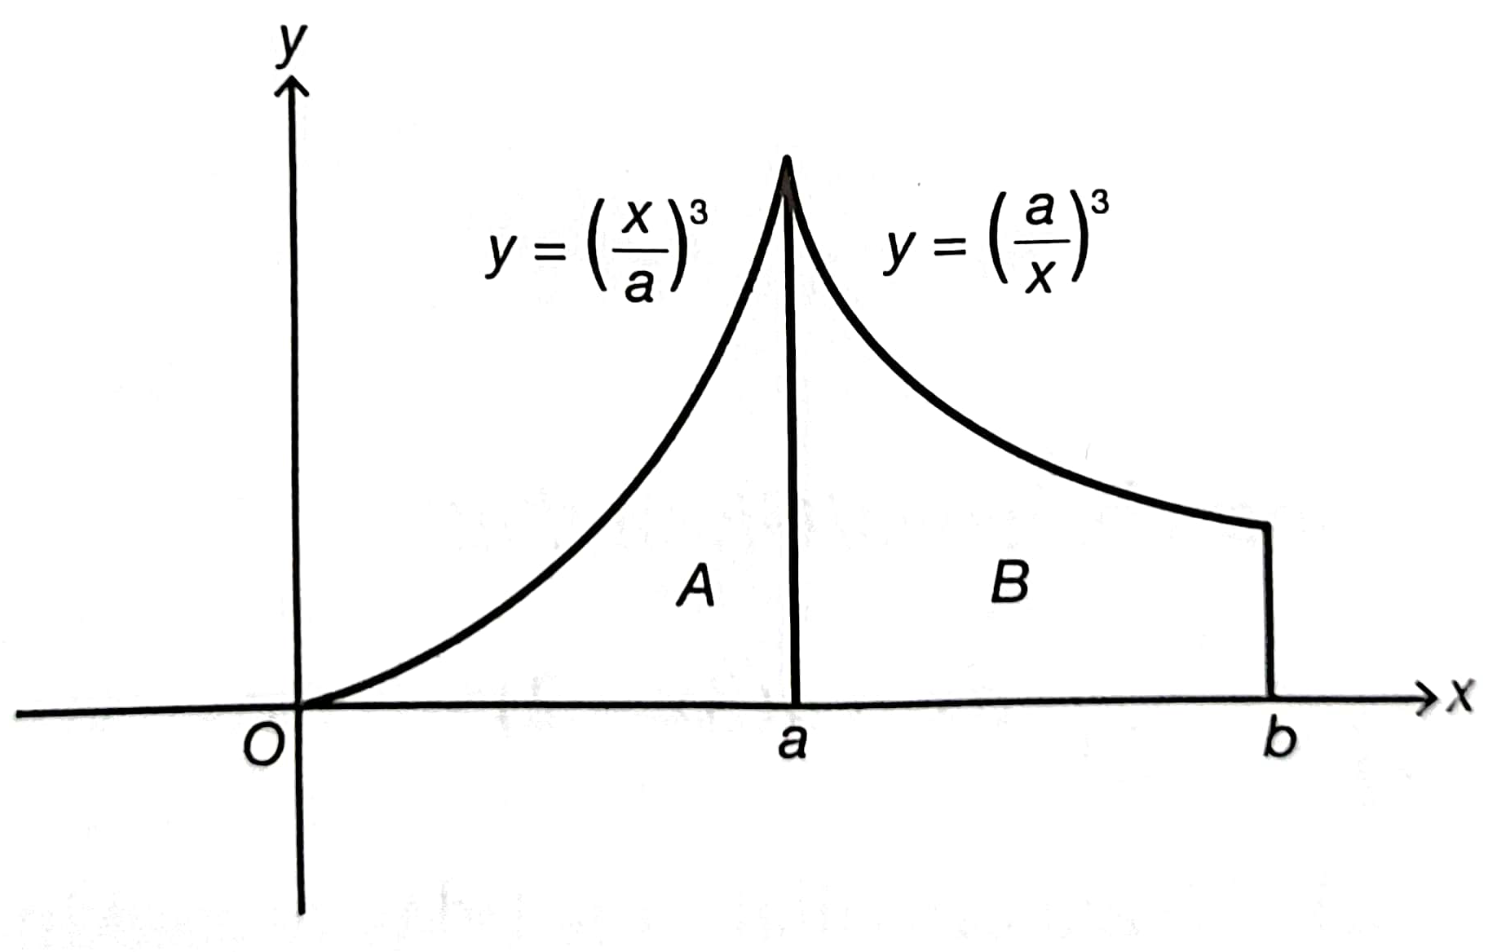
\includegraphics[width=0.36\textwidth]{images/27.png}
                  \end{center}
                  \begin{enumerate}
                        \item Find the area of the region $A$ in terms of $a$. \sol{}
                              \begin{flalign*}
                                    A_A & = \int_{0}^{a} {\left(\frac{x}{a}\right)}^3\,dx \\
                                        & =\int_{0}^{a} \frac{x^3}{a^3}\,dx               \\
                                        & = {\left[\frac{x^4}{4a^3}\right]}_{0}^{a}       \\
                                        & = \frac{a^4}{4a^3}                              \\
                                        & = \frac{a}{4} \eos
                              \end{flalign*}

                        \item Find the area of the region $B$ in terms of $a$ and $b$. \sol{}
                              \begin{flalign*}
                                    A_B & = \int_{a}^{b} {\left(\frac{a}{x}\right)}^3\,dx    \\
                                        & = a^3\int_{a}^{b} \frac{1}{x^3}\,dx                \\
                                        & = a^3{\left[-\frac{1}{2x^2}\right]}_{a}^{b}        \\
                                        & = a^3\left(-\frac{1}{2b^2} + \frac{1}{2a^2}\right) \\
                                        & = a^3\left(\frac{-a^2 + b^2}{2a^2b^2}\right)       \\
                                        & = \frac{ab^2 - a^3}{2b^2} \eos
                              \end{flalign*}

                        \item Show that \textit{the area of region} $A > \dfrac{1}{2}$ \textit{area of region
                                    $B$} for all values of $a$ and $b$ where $0 < a < b$. \sol{}
                              \begin{flalign*}
                                    A_A            & = \frac{a}{4}                          \\
                                    \frac{1}{2}A_B & = \frac{ab^2 - a^3}{4b^2}              \\
                                                   & = \frac{ab^2}{4b^2} - \frac{a^3}{4b^2} \\
                                                   & = \frac{a}{4} - \frac{a^3}{4b^2}
                              \end{flalign*}
                              \begin{flalign*}
                                    \forall\     & a,b \in \mathbb{R},\ 0 < a < b               \\
                                    \because\    & \frac{a}{4} > \frac{a}{4} - \frac{a^3}{4b^2} \\
                                    \therefore\  & A_A > \frac{1}{2}A_B \quad (shown)\eos
                              \end{flalign*}
                  \end{enumerate}

            \item Diagram below shows the cross-section of an anti-heat bowl which is made of
                  stainless steel. The bowl has two layers in which the space between the two
                  layers is a vacuum which functions as a heat insulator.
                  \begin{center}
                        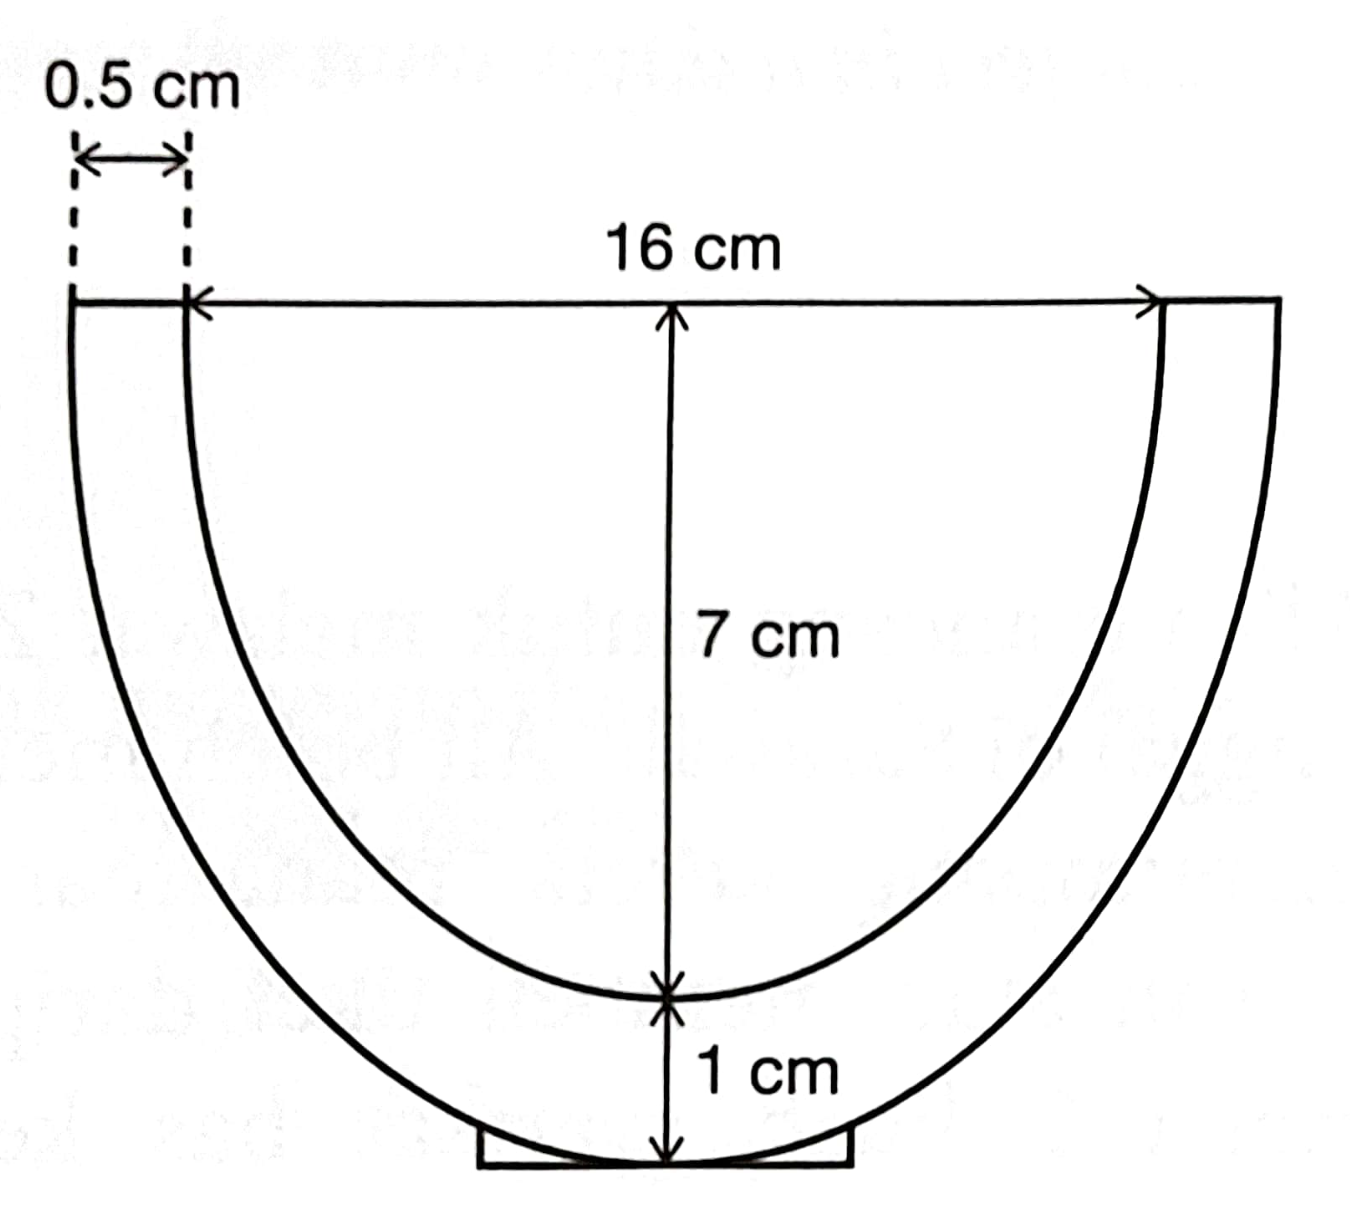
\includegraphics[width=0.36\textwidth]{images/28.png}
                  \end{center}
                  The inner and the outer layers of the bowl are parabolic in shape which are
                  represented by the equations $y = ax^2 + b$ and $y = \dfrac{32}{289}x^2$
                  respectively.
                  \begin{enumerate}
                        \item Find the values of $a$ and $b$. \sol{}
                              \begin{flalign*}
                                    y & = ax^2 + b                          \\
                                    b & = 1 \quad (\text{y-intercept}) \eos \\
                                    y & = ax^2 + 1
                              \end{flalign*}
                              The bowl is split into two equal parts by the y-axis, while the height of the bowl is $8$\textit{cm} Hence, the top-right corner of the bowl is $(8, 8)$.
                              \begin{flalign*}
                                    8   & = a(64) + 1         \\
                                    64a & = 7                 \\
                                    a   & = \frac{7}{64} \eos
                              \end{flalign*}

                        \item Anis wants to pour $1.5$ litres of milk into the bowl. Identify whether the
                              bowl can hold $1.5$ litres of milk. Justify your answer. \sol{}
                              \begin{flalign*}
                                    y         & = \frac{7}{64}x^2 + 1 \\
                                    64y       & = 7x^2 + 64           \\
                                    64y - 64  & = 7x^2                \\
                                    64(y - 1) & = 7x^2                \\
                                    x^2       & = \frac{64}{7}(y - 1)
                              \end{flalign*}
                              The volume of the bowl is
                              \begin{flalign*}
                                    V_x & = \int_1^7 \pi x^2\,dy                                                                     \\
                                        & = \pi\int_1^7 \frac{64}{7}(y - 1)\,dy                                                      \\
                                        & = \frac{64}{7}\pi\int_1^8 (y - 1)\,dy                                                      \\
                                        & = \frac{64}{7}\pi{\left[\frac{y^2}{2} - y\right]}_{1}^{8}                                  \\
                                        & = \frac{64}{7}\pi\left[\left(\frac{64}{2} - 8\right) - \left(\frac{1}{2} - 1\right)\right] \\
                                        & = \frac{64}{7}\pi\left(24 + \frac{1}{2}\right)                                             \\
                                        & = 224\pi                                                                                   \\
                                        & \approx 703.7168\textit{cm}^3                                                              \\
                                        & \approx 703.7168\textit{ml}
                              \end{flalign*}
                              Hence, the bowl is not capable of holding $1.5$ litres of milk due to insufficient volume. $\eos$
                  \end{enumerate}

            \item Diagram below shows parts of the curves $y = x^2 + 5x + 4$ and $y = 4 - x^2$.
                  \begin{center}
                        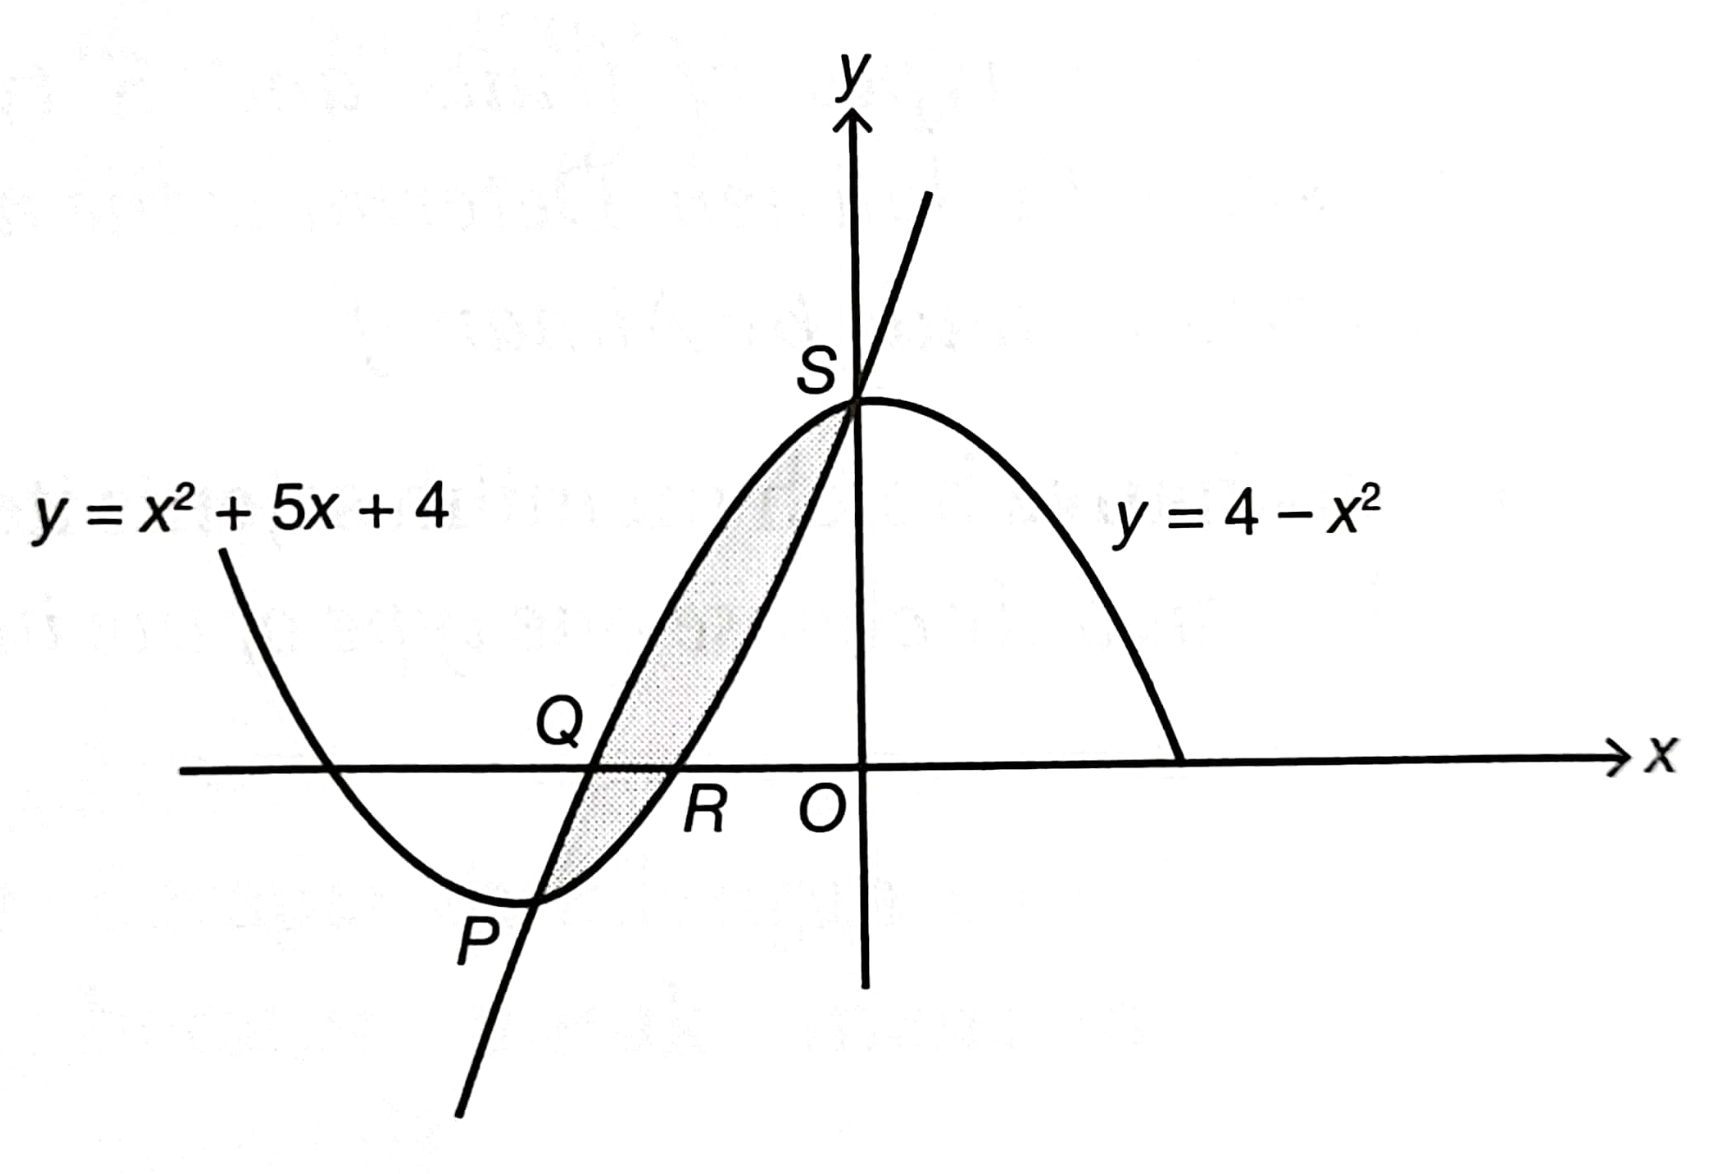
\includegraphics[width=0.36\textwidth]{images/29.png}
                  \end{center}
                  Find
                  \begin{enumerate}
                        \item the points of intersection $P$ and $S$. \sol{}
                              \begin{flalign*}
                                    x^2 + 5x + 4 & = 4 - x^2                    \\
                                    2x^2 + 5x    & = 0                          \\
                                    x(2x + 5)    & = 0                          \\
                                    x = 0        & \text{ or } x = -\frac{5}{2}
                              \end{flalign*}
                              \begin{flalign*}
                                    x = 0,\ y            & = 4 - 0^2 = 4                     \\
                                    x = -\frac{5}{2},\ y & = 4 - \left(-\frac{5}{2}\right)^2 \\
                                                         & = 4 - \frac{25}{4}                \\
                                                         & = -\frac{9}{4}
                              \end{flalign*}
                              Hence, the points of intersection are $S(0, 4)$ and $P(-\dfrac{5}{2}, -\dfrac{9}{4})$. $\eos$

                        \item the coordinates of the points $Q$ and $R$. \sol{}
                              \begin{flalign*}
                                    4 - x^2    & = 0               \\
                                    x^2 - 4    & = 0               \\
                                    (x+2)(x-2) & = 0               \\
                                    x = -2     & \text{ or } x = 2
                              \end{flalign*}
                              \begin{flalign*}
                                    \because\    & x_Q < 0,\ x_Q = -2 \\
                                    \therefore\  & Q(-2, 0) \eos
                              \end{flalign*}
                              \begin{flalign*}
                                    x^2 + 5x + 4   & = 0                \\
                                    (x + 1)(x + 4) & = 0                \\
                                    x = -1         & \text{ or } x = -4
                              \end{flalign*}
                              \begin{flalign*}
                                    \because\    & x_R > x_Q,\ x_R = -1 \\
                                    \therefore\  & R(-1, 0) \eos
                              \end{flalign*}

                        \item the area of the shaded region. \sol{}

                              Let the area above the $x$-axis be $A_A$ and the area below the $x$-axis be
                              $A_B$.
                              \begin{flalign*}
                                    A_A & = \int_{-2}^0 \left(4 - x^2\right)\,dx - \int_{-1}^0 \left(x^2 + 5x + 4\right)\,dx                                                       & \\
                                        & = {\left[4x - \frac{1}{3}x^3\right]}_{-2}^{0} - {\left[\frac{1}{3}x^3 + \frac{5}{2}x^2 + 4x\right]}_{-1}^{0}                             & \\
                                        & = \left[0 - \left(-8 + \frac{8}{3}\right)\right] - \left[0 - \left(-\frac{1}{3} + \frac{5}{2} - 4\right)\right]                          & \\
                                        & = \frac{16}{3} - \frac{11}{6}                                                                                                              \\
                                        & = 3\frac{1}{2} \textit{units}^2                                                                                                            \\
                                    A_B & = \left|\int_{-2.5}^{-1} \left(x^2 + 5x + 4\right)\,dx\right| - \left|\int_{-2.5}^{-2} \left(4 - x^2\right)\,\right.                       \\
                                        & \ \ \ \ \left.dx\right|                                                                                                                  & \\
                                        & = \left|\left[\frac{1}{3}x^3 + \frac{5}{2}x^2 + 4x\right]_{-2.5}^{-1}\right| - \left|\left[4x - \frac{1}{3}x^3\right]_{-2.5}^{-2}\right| & \\
                                        & = \left|\left[\left(-\frac{1}{3} + \frac{5}{2} - 4\right) - \left(-\frac{125}{24} + \frac{125}{8} - 10\right)\right]\right|                \\
                                        & \ \ \ \ - \left|\left[\left(-8 + \frac{8}{3}\right) - \left(-10 + \frac{125}{24}\right)\right]\right|                                      \\
                                        & = \left|\left(-\frac{11}{6} - \frac{5}{12}\right)\right| - \left|\left(-\frac{16}{3} + \frac{115}{24}\right)\right|                        \\
                                        & = \frac{9}{4} - \frac{13}{24}                                                                                                              \\
                                        & = 1\frac{17}{24} \textit{units}^2
                              \end{flalign*}
                              \begin{flalign*}
                                    A & = A_A + A_B                           \\
                                      & = 3\frac{1}{2} + 1\frac{17}{24}       \\
                                      & = 5\frac{5}{24} \textit{units}^2 \eos
                              \end{flalign*}
                  \end{enumerate}
      \end{enumerate}
\end{multicols*}

\end{document}